\documentclass[xcolor={usenames,dvipsnames,svgnames,table}]{beamer}

\mode<presentation>
\usetheme{Madrid}

\usecolortheme[RGB={80,0,0}]{structure}
\useoutertheme[subsection=false]{miniframes}
\useinnertheme{default}

% hide navigation controlls
\setbeamertemplate{navigation symbols}{}

\setbeamercolor{normal text}{fg=black}
\setbeamercovered{dynamic}
\beamertemplatetransparentcovereddynamicmedium
%\usepackage{chronology}
\setbeamertemplate{caption}[numbered]

\definecolor{Maroon}{RGB}{80,0,0}
\definecolor{BurntOrange}{RGB}{204,85,0}


% load macros and prevent authblk from loading
\makeatletter
% prevent a package from loading
\newcommand{\dontusepackage}[2][]{%
    \@namedef{ver@#2.sty}{9999/12/31}%
    \@namedef{opt@#2.sty}{#1}
}

% a macro to load packages only if they are not yet loaded, needed for combination of beamer and hyperref
\newcommand{\usepackagesave}[2][{}]{
    \ltx@ifpackageloaded{#2}{}{
        \usepackage[#1]{#2}}
}
\makeatother
\dontusepackage{authblk}

% load packages, settings and definitions
% this file contains all commonly used packages for the Rattlesnake documentation
% new package, add comment what they are used for

% command packages
\usepackage{xifthen}     % if -then else command

% language and font improvements
\usepackage[english]{babel}	% Multilingual support - https://www.ctan.org/pkg/babel
\usepackage[utf8]{inputenc} % Accept different input encodings - https://www.ctan.org/pkg/inputenc
\usepackage[kerning,spacing,babel]{microtype} % Subliminal refinements towards typographical perfection - https://www.ctan.org/pkg/microtype
\usepackage{eepic}      % Extensions to epic - https://www.ctan.org/pkg/eepic
\usepackage{epic}       % Enhance LaTeX picture mode - https://www.ctan.org/pkg/epic
\usepackage[T1]{fontenc} % selecting font encodingsselecting font encodings - https://www.ctan.org/pkg/fontenc
\usepackage{lmodern}

% title packages
\usepackage{authblk}		% footnote style author/affiliation - https://www.ctan.org/pkg/authblk

% symbols
\usepackage{upgreek}		% Upright Greek letters - https://www.ctan.org/pkg/upgreek
\usepackage{cancel}			% \cancel cmd - https://www.ctan.org/pkg/cancel

% chemical and isotope packages
\usepackage{isotope}		% isotope command - https://www.ctan.org/pkg/isotope
%\usepackage{mhchem}			% chemical formulae/equations - https://www.ctan.org/pkg/mhchem

% layout packages
\usepackage{xspace}			% smart space \xspace - https://www.ctan.org/pkg/xspace
\usepackage{icomma}			% smart math comma - https://www.ctan.org/pkg/icomma
\usepackage{chngpage}		% page layout change during document - https://www.ctan.org/pkg/chngpage
\usepackage[usenames,dvipsnames,svgnames,table]{xcolor}			% color definitions - https://www.ctan.org/pkg/xcolor
\usepackage{enumitem}   % layout for itemize and enumerate - http://www.ctan.org/pkg/enumitem
\usepackage{setspace}    % allows for \singlespacing, \onehalfspacing, and \doublespacing commands - https://www.ctan.org/pkg/setspace

% floating packages
% needed by the breakalgo environment labelsep=quad
\usepackage[singlelinecheck=false, labelsep=quad]{caption}	% table captions - https://www.ctan.org/pkg/caption
\usepackage{subcaption}		% Support for sub-captions - https://www.ctan.org/pkg/subcaption
\usepackage{placeins}   	% Control float placement - https://www.ctan.org/pkg/placeins
\usepackage{float}      	% Improved interface for floating objects - https://www.ctan.org/pkg/float

% table packages
\usepackage{supertabular}	% multi-page tables package - https://www.ctan.org/pkg/supertabular
\usepackage{booktabs}		% table settings - https://www.ctan.org/pkg/booktabs
\usepackage{array}			% Extending the array and tabular environments - https://www.ctan.org/pkg/array
\usepackage{multirow}		% tabular cells spanning multiple rows - https://www.ctan.org/pkg/multirow
% \usepackage{tabls}      % Better vertical spacing in tables and arrays - https://www.ctan.org/pkg/tabls
\usepackage{colortbl}      % Allows for color manipulation within tables - https://www.ctan.org/pkg/colortbl

% pictures, plots and listings
\usepackage{graphicx}		% include graphics - https://www.ctan.org/pkg/graphicx
\usepackage{wrapfig}		% wrapfigure enviroment - https://www.ctan.org/pkg/wrapfig
\usepackage{pgfplots}		% latex plots - https://www.ctan.org/pkg/pgfplots


% source code and algorithms
\usepackage{algorithmicx} % newer version of algorithmic - https://www.ctan.org/pkg/algorithmicx
\usepackage{listings} 	% source code listings - http://www.ctan.org/pkg/listings
\usepackage{verbatim}   % verbatim - https://www.ctan.org/pkg/verbatim

% misc packages
\usepackage{url}        % provide \url command for web addresses - https://www.ctan.org/pkg/url
\usepackage{import}			% Establish input relative to a directory - https://www.ctan.org/pkg/import
\usepackage{afterpage}  % Execute command after the next page break - https://www.ctan.org/pkg/afterpage
\usepackage{lscape}     % Place selected parts of a document in landscape - https://www.ctan.org/pkg/lscape
\usepackage{rotating}   % Rotation tools, including rotated full-page floats - https://www.ctan.org/pkg/rotating
\usepackage{chngcntr}   % Change the resetting of counters - http://ctan.org/pkg/chngcntr
\usepackage{textpos}    % Allows logo and banner manipulation

% eps support
\usepackage{epsfig}       % include eps figures - https://www.ctan.org/pkg/epsfig
\usepackage{epsf}          % Simple macros for EPS inclusion - https://www.ctan.org/pkg/epsf
\usepackage{epstopdf}   %use .eps images (as pdf) in \includegraphics


% reference packages
% hyperref must be loaded before amsmath to avoid problems with subequations and align
\usepackage{hyperref}		% Extensive support for hypertext - https://www.ctan.org/pkg/hyperref


% packages that must be loaded after hyperref - http://tex.stackexchange.com/questions/1863/which-packages-should-be-loaded-after-hyperref-instead-of-before
\usepackage{geometry}		% Flexible and complete interface to document dimensions - https://www.ctan.org/pkg/geometry
\usepackage{algorithm}  % algorithm enviroment

% ams math packages
\usepackage{amsmath}    % mathematical facilities - https://www.ctan.org/pkg/amsmath
\usepackage{amsfonts}   % fonts for math - https://www.ctan.org/pkg/amsfonts
\usepackage{amssymb}    %
\usepackage{amsthm}     % Typesetting theorems - https://www.ctan.org/pkg/amsthm

\usepackage{nameref}		% allows references with names instread of numbers \nameref - http://www.ctan.org/pkg/nameref
\usepackage[capitalize,nameinlink]{cleveref}   % smart references - http://ctan.org/pkg/cleveref

% general settings
\renewcommand\floatpagefraction{0.75} % threshold for floating objects to be placed on a page

\makeatletter
% center floats generally
\g@addto@macro\@floatboxreset\centering
% gives the current section name
\newcommand*{\currentname}{\@currentlabelname}
\makeatother

% figure setting, controlles the height of pgfplots from the main script
\newlength{\figheight}
\setlength{\figheight}{12cm}

% example for hyperref setup, we have to see if we can get that better
\hypersetup{
  linktocpage=true,       % links in table of contents
  bookmarks=true,         % show bookmarks bar?
  unicode=true,           % non-Latin characters in Acrobat's bookmarks
  pdftoolbar=true,        % show Acrobat's toolbar?
  pdfmenubar=true,        % show Acrobat's menu?
  pdffitwindow=false,     % window fit to page when opened
  pdfstartview={FitH},    % fits the width of the page to the window
  pdfnewwindow=true,      % links in new window
  colorlinks=false,       % false: boxed links; true: colored links
  linkcolor=red,          % color of internal links
  citecolor=green,        % color of links to bibliography
  filecolor=magenta,      % color of file links
  urlcolor=cyan,          % color of external links
  pdfborder={0 0 0},      % color of link frames
}


% set package versions
\pgfplotsset{compat=1.12}

% set table and figure counters here

% set up listings - see https://en.wikibooks.org/wiki/LaTeX/Source_Code_Listings
\lstset{ %
  backgroundcolor=\color{white},   % choose the background color; you must add \usepackage{color} or \usepackage{xcolor}; should come as last argument
  basicstyle=\footnotesize,        % the size of the fonts that are used for the code
  breakatwhitespace=false,         % sets if automatic breaks should only happen at whitespace
  breaklines=true,                 % sets automatic line breaking
  captionpos=b,                    % sets the caption-position to bottom
  commentstyle=\color{Gray},       % comment style
  deletekeywords={...},            % if you want to delete keywords from the given language
  escapeinside={\%*}{*)},          % if you want to add LaTeX within your code
  extendedchars=true,              % lets you use non-ASCII characters; for 8-bits encodings only, does not work with UTF-8
  frame=single,	                   % adds a frame around the code
  keepspaces=true,                 % keeps spaces in text, useful for keeping indentation of code (possibly needs columns=flexible)
  keywordstyle=\color{blue},       % keyword style
  morekeywords={*,...},            % if you want to add more keywords to the set
  numbers=left,                    % where to put the line-numbers; possible values are (none, left, right)
  numbersep=5pt,                   % how far the line-numbers are from the code
  numberstyle=\tiny\color{Gray},   % the style that is used for the line-numbers
  rulecolor=\color{black},         % if not set, the frame-color may be changed on line-breaks within not-black text (e.g. comments (green here))
  showspaces=false,                % show spaces everywhere adding particular underscores; it overrides 'showstringspaces'
  showstringspaces=false,          % underline spaces within strings only
  showtabs=false,                  % show tabs within strings adding particular underscores
  stepnumber=2,                    % the step between two line-numbers. If it's 1, each line will be numbered
  stringstyle=\color{mymauve},     % string literal style
  tabsize=2,	                     % sets default tabsize to 2 spaces
  title=\lstname                   % show the filename of files included with \lstinputlisting; also try caption instead of title
}

% define style for moose
\lstdefinestyle{cpp}{
  belowcaptionskip=1\baselineskip,
  breaklines=true,
  frame=TB,
  xleftmargin=\parindent,
  language=C,
  showstringspaces=false,
  basicstyle=\footnotesize\ttfamily,
  keywordstyle=\bfseries\color{green!40!black},
  commentstyle=\itshape\color{purple!40!black},
  identifierstyle=\color{blue},
  stringstyle=\color{orange},
}

\lstdefinestyle{python}{
  belowcaptionskip=1\baselineskip,
  breaklines=true,
  frame=,
  xleftmargin=\parindent,
  language=Python,
  showstringspaces=false,
  basicstyle=\footnotesize\ttfamily,
  keywordstyle=\bfseries\color{blue},
  commentstyle=\itshape\color{gray},
  identifierstyle=\color{black},
  stringstyle=\color{green},
}

\lstdefinelanguage{Moose}{
  morekeywords={one,two,three,four,five,six,seven,eight,
  nine,ten,eleven,twelve,o,clock,rock,around,the,tonight},
  sensitive=false,
  morecomment=[l]{//},
  morecomment=[s]{/*}{*/},
  morestring=[b]",
}

\lstdefinestyle{moose}{
  belowcaptionskip=1\baselineskip,
  breaklines=true,
  frame=tb,
  xleftmargin=\parindent,
  language=Moose,
  showstringspaces=false,
  basicstyle=\footnotesize\ttfamily,
  keywordstyle=\bfseries\color{blue},
  commentstyle=\itshape\color{gray},
  identifierstyle=\color{black},
  stringstyle=\color{green},
}

\lstset{literate=
  {á}{{\'a}}1 {é}{{\'e}}1 {í}{{\'i}}1 {ó}{{\'o}}1 {ú}{{\'u}}1
  {Á}{{\'A}}1 {É}{{\'E}}1 {Í}{{\'I}}1 {Ó}{{\'O}}1 {Ú}{{\'U}}1
  {à}{{\`a}}1 {è}{{\`e}}1 {ì}{{\`i}}1 {ò}{{\`o}}1 {ù}{{\`u}}1
  {À}{{\`A}}1 {È}{{\'E}}1 {Ì}{{\`I}}1 {Ò}{{\`O}}1 {Ù}{{\`U}}1
  {ä}{{\"a}}1 {ë}{{\"e}}1 {ï}{{\"i}}1 {ö}{{\"o}}1 {ü}{{\"u}}1
  {Ä}{{\"A}}1 {Ë}{{\"E}}1 {Ï}{{\"I}}1 {Ö}{{\"O}}1 {Ü}{{\"U}}1
  {â}{{\^a}}1 {ê}{{\^e}}1 {î}{{\^i}}1 {ô}{{\^o}}1 {û}{{\^u}}1
  {Â}{{\^A}}1 {Ê}{{\^E}}1 {Î}{{\^I}}1 {Ô}{{\^O}}1 {Û}{{\^U}}1
  {œ}{{\oe}}1 {Œ}{{\OE}}1 {æ}{{\ae}}1 {Æ}{{\AE}}1 {ß}{{\ss}}1
  {ű}{{\H{u}}}1 {Ű}{{\H{U}}}1 {ő}{{\H{o}}}1 {Ő}{{\H{O}}}1
  {ç}{{\c c}}1 {Ç}{{\c C}}1 {ø}{{\o}}1 {å}{{\r a}}1 {Å}{{\r A}}1
  {€}{{\euro}}1 {£}{{\pounds}}1
}

%% Common style and macro defintions for CLASS documents
%=================================================================================================

%%% General Commands

%% structural elements
% An explanation for a function
\newcommand{\explain}[1]{\mbox{\hspace{2em} #1}}
% attemtion box
\newcommand{\attention}[1]{\mbox{\hspace{2em} #1}}
% comments at the sde of the paragraph
\newcommand{\sidenotes}[1]{\marginpar{ {\footnotesize #1} }}
% create empty double page, TODO do we need that?
\newcommand{\clearemptydoublepage}{\newpage{\pagestyle{empty}\cleardoublepage}}
%TODO description here
\newcommand{\apost}{\textit{a posteriori\xspace}}
%TODO description here
\newcommand{\Apost}{\textit{A posteriori}\xspace}

%%% Math
%% Paratnhis etc.
% ()
\newcommand{\parenthesis}[1]{{\left(#1 \right)}}
% []
\newcommand{\bracket}[1]{{\left[ #1 \right]}}
% {}
\newcommand{\bracet}[1]{{\left\{#1 \right\}}}
% <>
\newcommand{\angled}[1]{{\left\langle#1\right\rangle}}

%% common math symbols
% imaginary number
\newcommand{\img}{\ensuremath{\hat{\imath}}\xspace}
% gradient symbol
\newcommand{\grad}{\vec{\nabla}}
\newcommand{\del}{\vec{\nabla}}
% adjoint
\newcommand{\adj}[2][{}]{{{#2}^{\dagger#1}}}
% order number
\newcommand{\order}[1]{^\parenthesis{#1}}
% iteration number
\newcommand{\iter}[1]{^{#1}}

%% common math function
% divergence
\renewcommand{\div}{\del\! \cdot \!}
% rotation
\newcommand{\rot}{\del\! \times \!}
% absolute value
\newcommand{\abs}[1]{\left|#1\right|}
% norm
\newcommand{\norm}[2][{}]{\lVert#2\rVert_{#1}}
% e function
\newcommand{\e}[1]{\mathrm{e}^{#1}}
% power of ten
\newcommand{\tento}[1]{\ensuremath{10^{#1}}\xspace}
% E notation
\newcommand{\E}[1]{\ensuremath{\cdot \tento{#1}}\xspace}
% sign
\DeclareMathOperator{\sign}{sign}

%% fraction
% 1 / 2
\newcommand{\half}[1][1]{\frac{#1}{2}}
% 1 / 3
\newcommand{\third}[1][1]{\frac{#1}{3}}
% 1 / 4
\newcommand{\fourth}[1][1]{\frac{#1}{4}}

% vectors etc
% vector, we use standard latex notation
% matrix
\newcommand{\mat}[1]{\mathbf{#1}}
% tensor
\newcommand{\tensor}[1]{\underline{\underline{#1}}}
% operator symbol
\newcommand{\op}[1]{\mathrm{\mathbf{#1}}}

% derivatives
% first derivatives
% general first derivative, with optional argument for f
\newcommand{\dd}[2][]{\frac{\partial #1}{\partial #2}}
% partial derivative for x, optional argument for f
\newcommand{\ddx}[1][]{\dd[#1]{x}}
% partial derivative for y, optional argument for f
\newcommand{\ddy}[1][]{\dd[#1]{y}}
% partial derivative for z, optional argument for f
\newcommand{\ddz}[1][]{\dd[#1]{z}}
% partial derivative for t, optional argument for f
\newcommand{\ddt}[1][]{\dd[#1]{t}}

% second derivatives, only for a single variable, cross derivatives are too many
% second general derivative, optional argument for f
\newcommand{\ddd}[2][{}]{\frac{\partial^2 #1}{\partial {#2}^2}}
% second partial derivative for x, optional argument for f
\newcommand{\ddxx}[1][]{\ddd[#1]{x}}
% second partial derivative for y, optional argument for f
\newcommand{\ddyy}[1][]{\ddd[#1]{y}}
% second partial derivative for z, optional argument for f
\newcommand{\ddzz}[1][]{\ddd[#1]{z}}
% second partial derivative for t, optional argument for f
\newcommand{\ddtt}[1][]{\ddd[#1]{t}}

% integrals
% integral dx, optional parameter for different variable
\newcommand{\dx}[1][x]{\,d#1}
% integral dy
\newcommand{\dy}{\dx[y]}
% integral dz
\newcommand{\dz}{\dx[z]}
% integral dt
\newcommand{\dt}{\dx[t]}
%integral dmu
\newcommand{\dmu}{\dx[\mu]}
%integral dOmega
\newcommand{\domg}{\dx[\direction]}

% spherical integrals
% shortcut for sphere notation
\newcommand{\sphere}{\ensuremath{\mathcal{S}}\xspace}
% angular quadrature weight
\newcommand{\aqweight}{\omega}

% integral over full sphere
\newcommand{\intsp}{\int_{4\pi}}
% integral over half sphere
\newcommand{\inthalfsp}{\int_{2\pi}}
% polar integral
\newcommand{\intpolar}{\int_{-1}^{1}}
% negative partial polar integral
\newcommand{\intnpolar}{\int_{-1}^{0}}
% positive partial polar integral
\newcommand{\intppolar}{\int_{0}^{1}}


% FEM symbols
% spatial domain
\newcommand*{\domain}{\ensuremath{\mathcal{D}}\xspace}
% boundary of a spatical domain
\newcommand*{\boundary}{\ensuremath{{\partial\domain}}\xspace}
% vacuum boundary of a spatical domain
\newcommand*{\vboundary}{\ensuremath{{\boundary}_v}\xspace}
% reflective boundary of a spatical domain
\newcommand*{\rboundary}{\ensuremath{{\boundary}_r}\xspace}
% interface surface
\newcommand*{\interface}{\ensuremath{{\Gamma}}\xspace}
% general and isotropic test function
\newcommand{\testfct}{\ensuremath{\phi^{*}}\xspace}
% angular test function
\newcommand{\atestfct}{\ensuremath{\psi^{*}}\xspace}
% surface normal
\newcommand{\normal}{\ensuremath{\vec{n}}\xspace}
% boundary normal
\newcommand{\bnormal}{\ensuremath{\normal_\mathrm{b}}\xspace}

% DFEM commands
% interface jump
\newcommand{\jump}[1]{[\![#1]\!]}
% what is the different?
\newcommand{\jmpa}[1]{[\![\![#1]\!]\!]}
% mean value
\newcommand{\meanval}[1]{\{\!\!\{#1\}\!\!\}}

% common physical symbols
% mass stream
\newcommand{\mdot}{\ensuremath{\dot{m}}\xspace}

% nuclear symbols
% Sn
\newcommand{\sn}[1][N]{\ensuremath{S_#1}\xspace}
% Pn
\newcommand{\pn}[1][N]{\ensuremath{P_#1}\xspace}
% keff
\newcommand{\keff}{\ensuremath{k_{\text{eff}}}\xspace}
% kinf
\newcommand{\kinf}{\ensuremath{k_{\text{inf}}}\xspace}

% transport symbols
\newcommand{\addgroup}[1]{\ifthenelse{\isempty{#1}}{}{_{#1}}}
% direction omega
\newcommand{\direction}{\ensuremath{\vec{\Omega}}\xspace}
% direction omega
\newcommand{\position}{\ensuremath{\vec{x}}\xspace}
% current
\newcommand{\current}[1][]{\ensuremath{\vec{J}\addgroup{#1}}\xspace}
% positive half range current
\newcommand{\ppcurrent}[1][]{\ensuremath{\hat{\jmath}\,^+\addgroup{#1}}\xspace}
% negative half range current
\newcommand{\npcurrent}[1][]{\ensuremath{\hat{\jmath}\,^-\addgroup{#1}}\xspace}
% drift vector
\newcommand{\drift}[1][]{\ensuremath{\hat{D}\addgroup{#1}}\xspace}
% local diffusion coefficient
\newcommand{\DC}[1][]{\ensuremath{\mathrm{D}\addgroup{#1}}\xspace}
% nonlocal diffusion tensor
\newcommand{\DCNL}[1][]{\ensuremath{\tensor{\mathrm{D}}\addgroup{#1}}\xspace}
% cross section label
\newcommand{\xslabel}[2][]{\ifthenelse{\isempty{#1}}{\mathrm{#2}}{\mathrm{#2},#1}}
% total cross section
\newcommand{\sigt}[1][]{\ensuremath{\sigma_{\xslabel[#1]{t}}}\xspace}
% scattering cross section
\newcommand{\sigs}[1][]{\ensuremath{\sigma_{\xslabel[#1]{s}}}\xspace}
% fission cross section
\newcommand{\sigf}[1][]{\ensuremath{\sigma_{\xslabel[#1]{f}}}\xspace}
% removal cross section
\newcommand{\sigr}[1][]{\ensuremath{\sigma_{\xslabel[#1]{r}}}\xspace}
% absorption cross section
\newcommand{\siga}[1][]{\ensuremath{\sigma_{\xslabel[#1]{a}}}\xspace}
% transport cross section
\newcommand{\sigtr}[1][]{\ensuremath{\sigma_{\xslabel[#1]{tr}}}\xspace}
% scattering moment
\newcommand{\sigl}[2][{}]{\ensuremath{\sigma_{#2#1}}\xspace}

% total cross section
\newcommand{\Sigt}[1][]{\ensuremath{\Sigma_{\xslabel[#1]{t}}}\xspace}
% scattering cross section
\newcommand{\Sigs}[1][]{\ensuremath{\Sigma_{\xslabel[#1]{s}}}\xspace}
% fission cross section
\newcommand{\Sigf}[1][]{\ensuremath{\Sigma_{\xslabel[#1]{f}}}\xspace}
% removal cross section
\newcommand{\Sigr}[1][]{\ensuremath{\Sigma_{\xslabel[#1]{r}}}\xspace}
% absorption cross section
\newcommand{\Siga}[1][]{\ensuremath{\Sigma_{\xslabel[#1]{a}}}\xspace}
% transport cross section
\newcommand{\Sigtr}[1][]{\ensuremath{\Sigma_{\xslabel[#1]{tr}}}\xspace}
% scattering moment
\newcommand{\Sigl}[2][{}]{\ensuremath{\Sigma_{#2#1}}\xspace}

% spatial weight function
\newcommand{\weight}[1][]{\ensuremath{w\addgroup{#1}}\xspace}

% physical units
% general style for a unit symbol
\newcommand{\unit}[1]{\mathrm{#1}}
% distance
% meter maybe \meter better and more clear?
\newcommand{\m}{\,\unit{m}\xspace}
% centimeter
\newcommand{\cm}{\,\unit{cm}\xspace}
% milimeter
\newcommand{\mm}{\,\unit{mm}\xspace}

% time
% second
\newcommand{\s}{\,\unit{s}\xspace}

% transport units
% scalar flux
\newcommand{\sfluxunit}{\,\ensuremath{\frac{1}{\unit{cm}^2\unit{s}}}\xspace}
% angular flux
\newcommand{\afluxunit}{\,\ensuremath{\frac{1}{\unit{cm}^2\unit{s}\cdot\unit{st}}}\xspace}
% diffusion coefficient
\newcommand{\dcunit}{\,\ensuremath{\unit{cm}}\xspace}


% \newenvironment{myverbatim}%            To change the pseudocode font
% {\par\noindent%
%  \rule[0pt]{\linewidth}{0.2pt}
%  \vspace*{-9pt}
%  \linespread{0.0}\small\verbatim}%
% {\rule[-5pt]{\linewidth}{0.2pt}\endverbatim}
%
% \newenvironment{myverbatim1}%            To change the pseudocode font
% {\par\noindent%
%  \rule[0pt]{\linewidth}{0.2pt}
%  \vspace*{-9pt}
%  \linespread{1.0}\scriptsize\verbatim}%
% {\rule[-5pt]{\linewidth}{0.2pt}\endverbatim}


\newcommand{\vr}{\vec{r}}
\newcommand{\vp}{\vec{p}}
\newcommand{\vOmega}{\vec{\Omega}}
\newcommand{\vJ}{\vec{J}}
\newcommand{\vO}{\vec{\Omega}}
\newcommand{\bra}{\left\langle}
\newcommand{\ket}{\right\rangle}
\newcommand{\sbra}{\left[}
\newcommand{\sket}{\right]}
\newcommand{\braSN}{\left\langle \! \left\langle}
\newcommand{\ketSN}{\right\rangle \! \right\rangle}
\newcommand{\sbraSN}{\left[ \! \left[}
\newcommand{\sketSN}{\right] \! \right]}
\renewcommand{\div}{\vec{\nabla} \cdot}
\newcommand{\grad}{\vec{\nabla}}
\newcommand{\vbeta}{\vec{\beta} }
\newcommand{\pdx}{\frac{\partial}{\partial x}}
\newcommand{\pdy}{\frac{\partial}{\partial y}}
\newcommand{\pdz}{\frac{\partial}{\partial z}}
\newcommand{\intrrr}{\int d^3 r \,}
\newcommand{\intrr}{\int d^2 r \,}
\newcommand{\dEdphi}{\partial_\phi E }
\newcommand{\dEdp}{\partial_p E }
\newcommand{\dBdphi}{\partial_\phi B }
\newcommand{\dBdp}{B }
\newcommand{\adj}{\phi^\dag}
\newcommand{\vefadj}{\varphi^\dag}
\newcommand{\surf}{\int_{\partial V}}
\newcommand{\domain}{V}
\newcommand{\bound}{\partial V}
\newcommand{\vn}{\vec{n}}
\newcommand{\Edd}{\mathbb{E}}
\newcommand{\BEdd}{B}
\newcommand{\sigt}{\sigma_t}
\newcommand{\sigs}{\sigma_s}
\newcommand{\siga}{\sigma_a}
%\newcommand{\isigt}{\sigma_t^{-1}}
%\newcommand{\isigtp}{\sigma_{t,p}^{-1}}
\newcommand{\isigt}{\ell_t}
\newcommand{\isigtp}{\ell_{t,p}}
\newcommand{\angSource}{\frac{q}{4 \pi}}
\newcommand{\angSourcep}{\frac{q_p}{4 \pi}}
\newcommand{\angSourcepd}{\frac{q+\delta q}{4 \pi}}
\newcommand{\angSourced}{\frac{\delta q}{4 \pi}}
\newcommand{\scalSource}{q}
\newcommand{\angResp}{q^\dag}
\newcommand{\scalResp}{q^\dag}
\newcommand{\qoi}{{\it QoI}\xspace}
\newcommand{\tcr}[1]{\textcolor{red}{#1}}
\newcommand{\tcb}[1]{\textcolor{blue}{#1}}
\newcommand{\tcm}[1]{\textcolor{magenta}{#1}}
\newcommand{\tcg}[1]{\textcolor{BlueGreen}{#1}}


% nicer item settings
\setlist[1]{nolistsep,label=\(\textcolor{Maroon}{\blacksquare}\)}
\setlist[2]{nolistsep,label=\(\textcolor{Maroon}{\bullet}\)}

\setenumerate[1]{
	label=\protect\usebeamerfont{enumerate item}%
	\protect\usebeamercolor[fg]{enumerate item}%
	\insertenumlabel.
}

%%%%%%%%%%%%%%%%%%%%%%%%%%%%%%%%%%%%%%%%%%%%%%%
%%% edit to fit your document

% set up pdf support and indexing
\hypersetup{
    pdftitle={Adjoint-Based Sensitivity for Radiation Transport Using an Eddington Tensor Formulation},
    pdfauthor={Ian Halvic},
}

\title[]{Adjoint-Based Sensitivity for Radiation Transport Using an Eddington Tensor Formulation}
\author[ ]{Ian Halvic}
\institute[Texas A\&M]{Department of Nuclear Engineering \\ Texas A\&M University}
\date[11/15/18]

\begin{document}

% title page, do not edit
{
\setbeamertemplate{headline}[default] 
\begin{frame}
\vspace{-1.1cm}
	\begin{figure}[t]
		\centering
			
\includegraphics[width=.25\textwidth]{figures2/seal.png}
	\end{figure}
\vspace{-0.75cm}
\titlepage
\end{frame}
}

%%%%%%%%%%%%%%%%%%%%%%%%%%%%%%%%%%%%%%%%%%%%%%%%%%%%%%%%%%%%%%%%%%%%%%%%%%%%%%%%%%%%%%%%%%%%%%%%%%%%%%%%%%%
\section{Introduction}	% define sections here, it is possible to get section slides automatically, but this is not enabled
\subsection{}	% we have to keep these to get the navigation
%%%%%%%%%%%%%%%%%%%%%%%%%%%%%%%%%%%%%%%%%%%%%%%%%%%%%%%%%%%%%%%%%%%%%%%%%%%%%%%%%%%%%%%%%%%%%%%%%%%%%%%%%%%

\begin{frame}[t]\frametitle{Motivation}
\begin{flushleft}
CERT (Center for Exascale Radiation Transport) - Focus on deterministic transport code which can scale to Exascale regime
\begin{itemize}
\item Potentially many unknowns for each transport solve
\item Initial focus was on time-dependent transport experiments with detector quantity of interest (\qoi)
\item High dimensionality of solution (space, angle, energy, and time) leads to memory limitations
\item UQ using adjoint transport is negatively affected by this limitation.
\item Can we get away with a Quasi-diffusive treatment with the adjoint approach to reduce dimensionality and still obtain the correct $\delta \qoi$ for use in UQ?
\end{itemize}
\end{flushleft}
\end{frame}
 
 %%%%%%%%%%%%%%%%%%%%%%%%%%%%%%%%%%%%%%%%%%%%%%%%%%%%%%%%%%%%%%%%%%%%%%%%%%%%%%%%%%%%%%%%%%%%%%%%%%%%%%%%%%%

%%%%%%%%%%%%%%%%%%%%%%%%%%%%%%%%%%%%%%%%%%%%%%%%%%%%%%%%%%%%%%%%%%%%%%%%%%%%%%%%%%%%%%%%%%%%%%%%%%%%%%%%%%%

%\begin{frame}[t]\frametitle{Motivation}
%\begin{flushleft}
%Adjoint methods provide a mechanism for propagating uncertainty in the system variables to the uncertainty in the desired \tcr{quantity of interest} (\qoi). 
%\vspace{2mm}
%In general adjoint methods 
%have the advantages
%\begin{itemize}
%\item No additional solves required to find the change in \tcr{\qoi, $\delta$\qoi}
%\item Change in \qoi is found using a simple inner product
%\end{itemize}
%\vspace{3mm}
%While adjoint methods can greatly reduce the number of system solves required for sensitivity calculations, \tcr{for transport} memory usage may become an issue. To compute $\delta \qoi$, adjoint transport requires storing both the forward angular $\psi$ and adjoint angular $\psi^\dag$ fluxes. This is prohibitive for \tcr{time-dependent transport} where angular fluxes must be stored \tcr{for each timestep}.
%\vspace{2mm}
%\begin{itemize}
%\item consider a \tcr{quasi-diffusion approach to reduce the dimensionality}, so only scalar fluxes are stored
%\end{itemize}
%\end{flushleft}
%\end{frame}
 
 %%%%%%%%%%%%%%%%%%%%%%%%%%%%%%%%%%%%%%%%%%%%%%%%%%%%%%%%%%%%%%%%%%%%%%%%%%%%%%%%%%%%%%%%%%%%%%%%%%%%%%%%%%%

\begin{frame}\frametitle{Approach}
\begin{flushleft}
\begin{itemize}
\item We consider a simple transport system
\begin{itemize}
\item steady state, 1 group
\item isotropic sources and response functions
\item isotropic scattering
\end{itemize}
\end{itemize}
\begin{itemize}
\item Present \tcr{transport} equation along with the \tcr{transport adjoint}
\item Formulate a \tcb{Variable Eddington Tensor (VET)} system from the transport equation and \tcb{corresponding adjoint}
\item Refine the VET method in two ways
\begin{itemize} 
\item First leveraging the transport adjoint
\item Second estimating Eddington perturbation
\end{itemize}
\end{itemize}
\end{flushleft}
\end{frame}

%%%%%%%%%%%%%%%%%%%%%%%%%%%%%%%%%%%%%%%%%%%%%%%%%%%%%%%%%%%%%%%%%%%%%%%%%%%%%%%%%%%%%%%%%%%%%%%%%%%%%%%
%%%%%%%%%%%%%%%%%%%%%%%%%%%%%%%%%%%%%%%%%%%%%%%%%%%%%%%%%%%%%%%%%%%%%%%%%%%%%%%%%%%%%%%%%%%%%%%%%%%%%%%%%%%

\begin{frame}\frametitle{\qoi Computed Using Transport}
 \begin{flushleft}
To begin, consider the one-group steady state transport system with isotropic source $q$ and scattering $\sigs$
\begin{subequations}
\begin{equation}
\label{SNfwd}
 \vO \cdot \grad \psi + \sigt \psi = \frac{\sigs}{4 \pi} \phi + \angSource
\end{equation}
\begin{equation}
\psi(\vr) = \psi^{ \text{inc}}(\vr) \quad \vr \in \partial V^{-} = \{  \vr \in \bound , \quad \vO \cdot \vec{n} < 0 \}
\end{equation}
\end{subequations}
We are concerned with a volumetric and isotropic \qoi given by $\scalResp$
\begin{equation}
\begin{split}
\qoi 	
&:= \braSN \psi , \tcr{\scalResp} \ketSN \equiv \int_V \int_\Omega \psi \scalResp \, d\Omega dV \\
&= \bra \phi , \scalResp \ket \equiv \int_V \phi \scalResp \, dV \\
\end{split}
\end{equation} 
\end{flushleft}
\end{frame}

%%%%%%%%%%%%%%%%%%%%%%%%%%%%%%%%%%%%%%%%%%%%%%%%%%%%%%%%%%%%%%%%%%%%%%%%%%%%%%%%%%%%%%%%%%%%%%%%%%%%%%%%%%%
\section{Formulations}	% define sections here, it is possible to get section slides automatically, but this is not enabled
\subsection{}	% we have to keep these to get the navigation
%%%%%%%%%%%%%%%%%%%%%%%%%%%%%%%%%%%%%%%%%%%%%%%%%%%%%%%%%%%%%%%%%%%%%%%%%%%%%%%%%%%%%%%%%%%%%%%%%%%%%%%%%%%


 %%%%%%%%%%%%%%%%%%%%%%%%%%%%%%%%%%%%%%%%%%%%%%%%%%%%%%%%%%%%%%%%%%%%%%%%%%%%%%%%%%%%%%%%%%%%%%%%%%%%%%%%%%%
% %%%%%%%%%%%%%%%%%%%%%%%%%%%%%%%%%%%%%%%%%%%%%%%%%%%%%%%%%%%%%%%%%%%%%%%%%%%%%%%%%%%%%%%%%%%%%%%%%%%%%%%%%%%
%
%\begin{frame}\frametitle{Sensitivity Using Forward Transport}
% \begin{flushleft}
%This presents the most straightforward (and most expensive) way to determine the change in the \qoi due to perturbations in the system parameters
%\begin{subequations}
%\begin{equation}
%\label{SNfwdp}
%\vO \cdot \grad \psi_{\tcr{p}} + ( \sigt + \tcb{\delta \sigt}) \psi_{\tcr{p}} = \frac{\sigs+ \tcb{\delta \sigs}}{4 \pi} \phi_{\tcr{p}} + \frac{q + \tcb{\delta q}}{4 \pi}
%\end{equation}
%\begin{equation}
%\psi(\vr) = \psi_{\tcr{p}}^{ \text{inc}}(\vr) \quad \vr \in \partial V^{-} = \{  \vr \in \bound , \quad \vO \cdot \vec{n} < 0 \}
%\end{equation}
%\end{subequations}
%Leading to the simple result
%\begin{equation}
%\delta \qoi = \bra \phi_{\tcr{p}} , \scalResp \ket - \bra \phi , \scalResp \ket = \bra \delta \phi , \scalResp \ket 
%\end{equation} 
%\end{flushleft}
%\end{frame}
%
% %%%%%%%%%%%%%%%%%%%%%%%%%%%%%%%%%%%%%%%%%%%%%%%%%%%%%%%%%%%%%%%%%%%%%%%%%%%%%%%%%%%%%%%%%%%%%%%%%%%%%%%%%%%
 
 
 %%%%%%%%%%%%%%%%%%%%%%%%%%%%%%%%%%%%%%%%%%%%%%%%%%%%%%%%%%%%%%%%%%%%%%%%%%%%%%%%%%%%%%%%%%%%%%%%%%%%%%%%%%%

\begin{frame}\frametitle{Transport Adjoint and \qoi}
 \begin{flushleft}
To avoid a forward solve for every perturbation case, an adjoint method may be employed.\cite{Marchuk} The adjoint system is defined 
\begin{subequations}
\begin{equation}
- \vO \cdot \grad \psi^\dag + \sigt \psi^\dag = \frac{\sigs}{4 \pi} \phi^\dag + \scalResp
\end{equation}
\begin{equation}
\psi^\dag(\vr) = \psi^{\dag \text{out}}(\vr)=0 \quad \vr \in \partial V^{+} = \{  \vr \in \bound , \quad \vO \cdot \vec{n} > 0 \}
\end{equation}
\end{subequations}
Through the standard adjoint method a surface term is added in the \qoi
\begin{equation}
\begin{split}
\qoi 
&= \bra \phi^\dag , \angSource \ket - \oint_{\partial V} \int_\Omega (\vO \cdot \vn) \psi^\dag  \psi \, d\Omega dS \\
&= \bra \phi^\dag , \angSource \ket - \sbraSN \psi^\dag , \psi \sketSN \\
\end{split}
\end{equation} 
\end{flushleft}
\end{frame}

 %%%%%%%%%%%%%%%%%%%%%%%%%%%%%%%%%%%%%%%%%%%%%%%%%%%%%%%%%%%%%%%%%%%%%%%%%%%%%%%%%%%%%%%%%%%%%%%%%%%%%%%%%%%\\
  %%%%%%%%%%%%%%%%%%%%%%%%%%%%%%%%%%%%%%%%%%%%%%%%%%%%%%%%%%%%%%%%%%%%%%%%%%%%%%%%%%%%%%%%%%%%%%%%%%%%%%%%%%%

%\begin{frame}\frametitle{Sensitivity Using Adjoint Transport}
% \begin{flushleft}
% Multiply by the perturbed $\psi_p$ by $\scalResp$ and integrate. First-order approximation used on last step.
%\begin{equation}
%\label{snSensPart}
%\begin{split}
%\qoi_p 
%&:=\braSN \psi_p , \tcg{\angResp} \ketSN \\
%&=\braSN \psi_p , \tcg{- \vO \cdot \grad \psi^\dag + \sigt \psi^\dag - \frac{\sigs}{4 \pi} \phi^\dag  }\ketSN \\
%&=\braSN  \vO \cdot \grad \psi_p + \sigt \psi_p - \frac{\sigs}{4 \pi} \phi_p , \psi^\dag  \ketSN - \sbraSN \psi_p, \psi^\dag \sketSN \\
%&= \braSN \tcm{ \vO \cdot \grad \psi_p + \sigma_{t,p}\psi_p} - \delta\sigt \tcr{\psi_p} \tcm{- \frac{\sigma_{s,p}}{4 \pi} \phi_p}
%+\frac{\delta \sigs}{4 \pi} \tcr{\phi_p}
% , \psi^\dag  \ketSN - \sbraSN \psi_p, \psi^\dag \sketSN \\
%&\tcr{\approx} \braSN \tcm{ \angSourcepd } - \delta\sigt \tcb{\psi} + \frac{\delta \sigs}{4 \pi} \tcb{\phi}
% , \psi^\dag  \ketSN - \sbraSN \psi_p, \psi^\dag \sketSN
%\end{split}
%\end{equation}
%
%\end{flushleft}
%\end{frame}

 %%%%%%%%%%%%%%%%%%%%%%%%%%%%%%%%%%%%%%%%%%%%%%%%%%%%%%%%%%%%%%%%%%%%%%%%%%%%%%%%%%%%%%%%%%%%%%%%%%%%%%%%%%%
 \begin{frame}\frametitle{Transport Adjoint}
 \begin{flushleft}
Perform $\qoi_p - \qoi$ to obtain the change in $\qoi$
\begin{equation}
\label{snSens}
\begin{split}
\delta \qoi 
&\approx \braSN  \angSourced - \delta\sigt\psi + \frac{\delta \sigs}{4 \pi} \phi
 , \psi^\dag  \ketSN - \sbraSN \delta \psi, \psi^\dag \sketSN \\
 &= \bra \angSourced, \phi^\dag \ket - \tcr{\braSN \delta\sigt\psi , \psi^\dag \ketSN} + \bra \frac{\delta \sigs}{4 \pi} \phi
 , \phi^\dag \ket - \sbraSN \delta \psi^{\text{inc}}, \psi^\dag \sketSN \\
\end{split}
\end{equation}
Pros
\begin{itemize}
\item Do not need SN solve for each perturbation scenario, just 2 SN solves to get unperturbed fluxes $\psi$ and $\psi^\dag$
\item Still exact for source (volumetric and boundary) perturbations, $\delta q$ and $\delta \psi^{\text{inc}}$
\end{itemize}
Cons
\begin{itemize}
\item Only first-order perturbation accurate ($\delta \sigs \delta \phi=0$, $\delta \sigt \delta \phi=0$)
\item Need to store angular dependent $\psi$ and $\psi^\dag$, which is prohibitive for time-dependent problems
\end{itemize}
\end{flushleft}
\end{frame}

% %%%%%%%%%%%%%%%%%%%%%%%%%%%%%%%%%%%%%%%%%%%%%%%%%%%%%%%%%%%%%%%%%%%%%%%%%%%%%%%%%%%%%%%%%%%%%%%%%%%%%%%%%%%
% %%%%%%%%%%%%%%%%%%%%%%%%%%%%%%
%
%\begin{frame}\frametitle{VET Formulation}
%\begin{flushleft}
%\begin{figure}[H]
%\label{Trial1}
%\centering
%  \centering
%  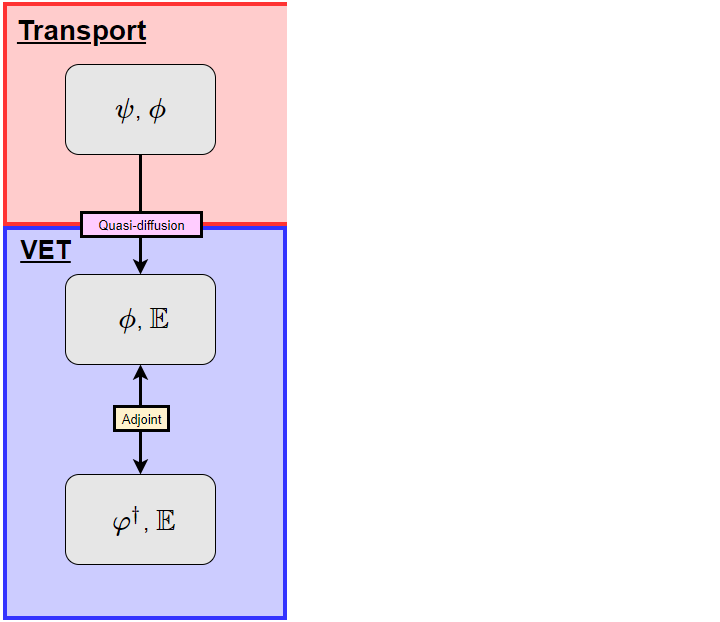
\includegraphics[scale=0.4]{figures2/BigRoadMap2.png}
%\end{figure}
%\end{flushleft}
%\end{frame}
%
%%%%%%%%%%%%%%%%%%%%%%%%%%%%%%%%%%%%%%%%%%%%%%%%%%%%%%%%%%%%%%%%%%%%%%%%
 %%%%%%%%%%%%%%%%%%%%%%%%%%%%%%%%%%%%%%%%%%%%%%%%%%%%%%%%%%%%%%%%%%%%%%%%%%%%%%%%%%%%%%%%%%%%%%%%%%%%%%%%%%%

\begin{frame}\frametitle{VET Formulation}
 \begin{flushleft}
Formulate the P1 equations and define an Eddington Tensor $\Edd$ and a Boundary Eddington Factor $\BEdd$ 
\begin{equation}
\div \vec{J} + (\sigt-\sigs) \phi = \scalSource
, \quad \quad 
\div \left(  \int d\Omega \vO \vO \psi \right) + \sigt \vec{J} = 0 
\end{equation}
\begin{equation}
\Edd(\vr)=\frac{\int d\Omega \vO \vO \psi(\vr,\vO)}{\phi(\vr)}
, \, \vr \in V \quad \quad 
\BEdd(\vr) = \frac{\int_{4 \pi} d\Omega \, | \vO \cdot \vn | \psi}{\phi(\vr)} , \, \vr \in \bound
\end{equation}
Combine into the VET formulation \cite{Miften}
\begin{subequations}
\begin{equation}
\label{VEFForm}
- \div \left( \frac{1}{\sigt}\div \Edd \phi \right) + \siga \phi = \scalSource \, \quad \vr \in V 
\end{equation}
\begin{equation}
2 J^{\text{inc}} = \BEdd \phi + \vn \cdot \frac{1}{\sigt} \div \Edd \phi \,\quad  \vr \in \bound
\end{equation}
\end{subequations}
If $\Edd$ and $\BEdd$ are known, then $\phi^{\text{VET}} = \phi^{\text{SN}}$
\end{flushleft}
\end{frame}

%%%%%%%%%%%%%%%%%%%%%%%%%%%%%%%%%%%%%%%%%%%%%%%%%%%%%%%%%%%%%%%%%%%%%%%%%%%%%%%%%%%%%%%%%%%%%%%%%%%%%%%%%%%
%%%%%%%%%%%%%%%%%%%%%%%%%%%%%%%%%%%%%%%%%%%%%%%%%%%%%%%%%%%%%%%%%%%%%%%%%%%%%%%%%%%%%%%%%%%%%%%%%%%%%%%%%%%
%
%\begin{frame}\frametitle{VET Adjoint Formulation}
% \begin{flushleft}
%To derive an expression for the VET adjoint equation $\vefadj$, start with the forward VET balance equation, Eq.~\eqref{VEFForm}
%\begin{equation}
%\label{VEFadjFormDeriv}
%\begin{split}
%\bra \scalSource , \vefadj \ket &= - \bra \div \left( \frac{1}{\sigt}\div \Edd \phi \right), \vefadj \ket +  \bra \siga \phi, \vefadj \ket   \\
%&= \bra \frac{1}{\sigt}\div \Edd \phi, \grad \vefadj \ket  +  \bra  \phi, \siga \vefadj \ket - \sbra \vn \cdot \frac{1}{\sigt}\div \Edd \phi, \vefadj \sket   \\
% &=  \bra \phi, \tcb{\Edd : \left( - \grad \left( \frac{1}{\sigt}\grad \vefadj \right) \right) + \siga \vefadj } \ket \\
% & - \sbra \vn \cdot  \frac{1}{\sigt}\div \Edd \phi, \vefadj \sket + \sbra \phi, \vn \cdot  \Edd \cdot \frac{1}{\sigt} \grad \vefadj \sket \\
%\end{split}
%\end{equation}
%Where the inner product $\sbra f ,g \sket = \oint_{\partial V} fg \, dS$ has been defined
%\end{flushleft}
%\end{frame}

 %%%%%%%%%%%%%%%%%%%%%%%%%%%%%%%%%%%%%%%%%%%%%%%%%%%%%%%%%%%%%%%%%%%%%%%%%%%%%%%%%%%%%%%%%%%%%%%%%%%%%%%%%%%
 %%%%%%%%%%%%%%%%%%%%%%%%%%%%%%%%%%%%%%%%%%%%%%%%%%%%%%%%%%%%%%%%%%%%%%%%%%%%%%%%%%%%%%%%%%%%%%%%%%%%%%%%%%%

\begin{frame}\frametitle{VET Adjoint Formulation}
 \begin{flushleft}
From the previous balance equation, an obvious form of the VET adjoint emerges
\begin{subequations}
\begin{equation}
\label{adjForm}
- \Edd : \left( \grad \left( \frac{1}{\sigt}\grad \vefadj \right) \right) + \siga \vefadj = \scalResp,    \quad \vr \in V
\end{equation}
\begin{equation}
\label{adjVETBC}
2J^{\dag,\text{out}} = B \vefadj+ \vn \cdot
\Edd \cdot \frac{1}{\sigma_{t} } \vec{\nabla} \vefadj,    \quad \vr \in \bound
\end{equation}
\end{subequations}
Choosing $J^{\dag,\text{out}} =0$ results in the relatively simple \qoi expression using this new formulation
\begin{equation}
\label{adjVETqoi}
\qoi=\bra \scalSource , \vefadj \ket  + \sbra \vefadj, 2J^{\text{inc}} \sket
\end{equation}
Note that $ \phi^\dag \neq \vefadj$
\end{flushleft}
\end{frame}

 %%%%%%%%%%%%%%%%%%%%%%%%%%%%%%%%%%%%%%%%%%%%%%%%%%%%%%%%%%%%%%%%%%%%%%%%%%%%%%%%%%%%%%%%%%%%%%%%%%%%%%%%%%%

 %%%%%%%%%%%%%%%%%%%%%%%%%%%%%%%%%%%%%%%%%%%%%%%%%%%%%%%%%%%%%%%%%%%%%%%%%%%%%%%%%%%%%%%%%%%%%%%%%%%%%%%%%%%

\begin{frame}\frametitle{Sensitivity Using VET Adjoint}
 \begin{flushleft}
Now an assumption is made that the \tcr{$\Edd$ and $\BEdd$ remain unperturbed under system perturbation}. Note $\ell_t = \frac{1}{\sigt}$
\begin{equation}
\label{VETSensDeriv}
\begin{split}
\qoi_p = &\bra \tcb{\phi_p} , \scalResp \ket \\
       = &\bra \tcb{\phi_p} , - \Edd : \left( \grad \isigt \grad \varphi^\dag \right) + \siga \vefadj \ket \\
\tcr{\approx} & \bra \scalSource + \delta \scalSource + \div \delta \isigt \div \left( \Edd \tcr{\phi} \right) - \delta \siga \tcr{\phi}, \vefadj \ket - \sbra \tcb{\phi_p}, \Edd \cdot \isigt \grad \vefadj \sket \\
&+ \sbra \vefadj, \isigt \div \Edd \tcb{\phi_p} \sket \\
=& \bra q, \vefadj \ket  + \bra \delta \scalSource + \div \delta \isigt \div \left( \Edd \tcr{\phi} \right)  - \delta \siga \tcr{\phi}, \vefadj \ket \\
& - \sbra \tcb{\phi_p}, \Edd \cdot \isigt \grad \vefadj \sket + \sbra \vefadj, \isigt \div \Edd \tcb{\phi_p} \sket 
\end{split}
\end{equation}

\end{flushleft}
\end{frame}

 %%%%%%%%%%%%%%%%%%%%%%%%%%%%%%%%%%%%%%%%%%%%%%%%%%%%%%%%%%%%%%%%%%%%%%%%%%%%%%%%%%%%%%%%%%%%%%%%%%%%%%%%%%%

  %%%%%%%%%%%%%%%%%%%%%%%%%%%%%%%%%%%%%%%%%%%%%%%%%%%%%%%%%%%%%%%%%%%%%%%%%%%%%%%%%%%%%%%%%%%%%%%%%%%%%%%%%%%

\begin{frame}\frametitle{Sensitivity Using VET Adjoint}
 \begin{flushleft}
 Subtracting off the unperturbed \qoi in Eq.~\eqref{adjVETqoi} and cleaning up some boundary terms results in
 \begin{equation}
\label{VETsens}
\begin{split}
\delta \qoi =&  \bra \delta \scalSource - \delta \siga \phi, \vefadj \ket  - \bra \delta \isigt \div \left( \Edd \phi \right) , \grad \vefadj \ket + \sbra \vefadj, 2 \delta J^{\text{inc}} \sket \\
\end{split}
\end{equation}
Pros
\begin{itemize}
\item Requires only 1 SN solve to get $\Edd$ and $\phi$, and 1 scalar VET solve for $\varphi^\dag$
\item No angular fluxes stored, only $\Edd$
\end{itemize}
Cons
\begin{itemize}
\item Only first order perturbation accurate (as was SN adjoint)
\item Major assumption that $\delta \Edd=0$, which is not always true. This means that the method in general is not exact for source perturbations $\delta q$ and $\delta \psi^{\text{inc}}$, which was the case for transport
\end{itemize}
\end{flushleft}
\end{frame}
 %%%%%%%%%%%%%%%%%%%%%%%%%%%%%%%%%%%%%%%%%%%%%%%%%%%%%%%%%%%%%%%%%%%%%%%%%%%%%%%%%%%%%%%%%%%%%%%%%%%%%%%%%%%

\begin{frame}\frametitle{Refinement Option 1: ``Blended'' Approach}
 \begin{flushleft}
Form a $\delta \qoi$ inner-product by picking the exact source terms from \tcr{SN adjoint Eq.~\eqref{snSens}} and cross-section terms from \tcb{VET formulation adjoint Eq.~\eqref{VETsens}}
\begin{equation}
\label{Blendsens}
\begin{split}
\delta \qoi =&  \tcr{\bra \angSourced , \phi^\dag \ket} \tcb{- \bra \delta \siga \phi, \vefadj \ket - \bra \delta \isigt \div \left( \Edd \phi \right) , \grad \vefadj \ket} \tcr{
- \sbraSN \delta \psi^\text{inc}, \psi^\dag \sketSN }\\
\end{split}
\end{equation}
Pros
\begin{itemize}
\item Requires 2 transport solves to get $\Edd$, $\phi$ and $\phi^\dag$ then one VET solve for $\varphi^\dag$
\item No angular fluxes stored
\item Still exact for source perturbations (equivalent to transport adjoint)
\end{itemize}
Cons
\begin{itemize}
%\item Lacks rigorous derivation
\item Could experience issues when both source and cross-section perturbation are present, compared to pure VET adjoint
\end{itemize}
\end{flushleft}
\end{frame}

%%%%%%%%%%%%%%%%%%%%%%%%%%%%%%%%%%%%%%%%%%%%%%%%%%%%%%%%%%%%%%%%%%%%%%%%%%%%%%%%%%%%%%%%%%%%%%%%%%%%%%%%%%%
 
%%%%%%%%%%%%%%%%%%%%%%%%%%%%%%%%%%%%%%%%%%%%%%%%%%%%%%%%%%%%%%%%%%%%%%%%%%%%%%%%%%%%%%%%%%%%%%%%%%%%%%%%%%%

\begin{frame}\frametitle{Refinement Option 2: Estimate $\delta \Edd$}
 \begin{flushleft}
Attempt to approximate by taking the slope with respect to perturbation parameters $\vp$
\begin{equation}
\delta \Edd \approx \frac{\partial \Edd}{\partial \vp} \cdot \delta \vp \approx \left( \frac{\Edd(\vp_1) - \Edd(\vp_0)}{\vp_1 - \vp_0} \right) \cdot \delta \vp
\end{equation}
 \begin{equation}
\label{VETsens}
\begin{split}
\delta \qoi =&  \bra \delta \scalSource - \delta \siga \phi, \vefadj \ket  - \bra \delta \isigt \div \left( \Edd \phi \right) , \grad \vefadj \ket + \sbra \vefadj, 2 \delta J^{\text{inc}} \sket \\
& - \bra  \isigt \div \left( \tcr{\delta \Edd} \phi \right), \grad \vefadj \ket
- \sbra \vefadj, \phi \tcr{\delta \BEdd} \sket
\end{split}
\end{equation}
Pros
\begin{itemize}
\item Attempts to resolve errors from the $\delta \Edd = 0$ assumption in VET adjoint
\end{itemize}
Cons
\begin{itemize}
\item Requires an additional transport solve for $\Edd(\vp_1)$. Pointless for only testing one perturbation scenario, potentially powerful for testing many perturbation scenarios
\end{itemize}
\end{flushleft}
\end{frame}

 %%%%%%%%%%%%%%%%%%%%%%%%%%%%%%%%%%%%%%%%%%%%%%%%%%%%%%%%%%%%%%%%%%%%%%%%%%%%%%%%%%%%%%%%%%%%%%%%%%%%%%%%%%%
 %%%%%%%%%%%%%%%%%%%%%%%%%%%%%%%
% %%%%%%%%%%%%%%%%%%%%%%%%%%%%%%
%
%\begin{frame}\frametitle{Adjoint-VET (Alternate VET)}
%\begin{flushleft}
%\begin{figure}[H]
%\label{Trial1}
%\centering
%  \centering
%  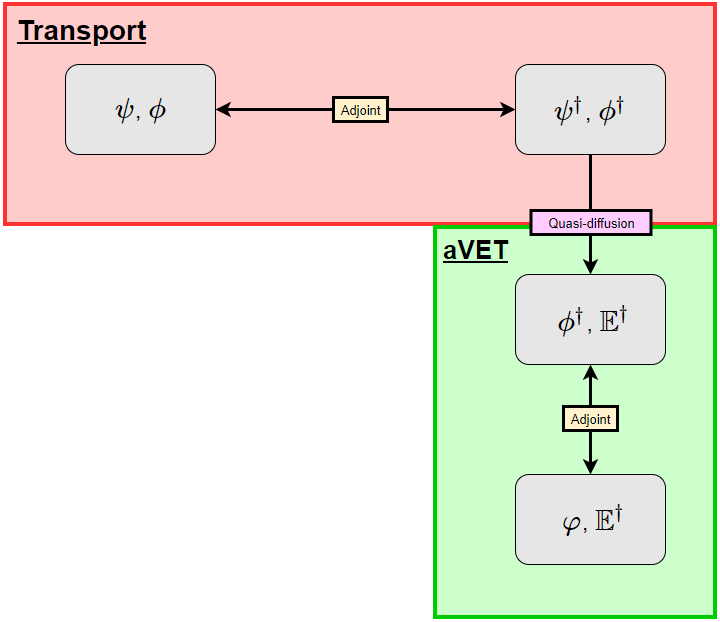
\includegraphics[scale=0.4]{figures2/BigRoadMap3.png}
%\end{figure}
%\end{flushleft}
%\end{frame}
%
%%%%%%%%%%%%%%%%%%%%%%%%%%%%%%%%%%%%%%%%%%%%%%%%%%%%%%%%%%%%%%%%%%%%%%%%
% %%%%%%%%%%%%%%%%%%%%%%%%%%%%%%%%%%%%%%%%%%%%%%%%%%%%%%%%%%%%%%%%%%%%%%%%%%%%%%%%%%%%%%%%%%%%%%%%%%%%%%%%%%%
%
%\begin{frame}\frametitle{Adjoint-VET (aVET)}
%\begin{flushleft}
%Reverse the order of the VET derivation, start with \tcr{adjoint} P1 and work towards an alternate forward $\varphi$
%\begin{equation}
%\label{0amAlt}
%\tcr{-}\div \vec{J}^\dag + (\sigt-\sigs) \phi^\dag  = \tcr{4\pi} \scalResp 
%, \quad \quad 
%\tcr{-}\div \left(  \int d\Omega \vO \vO \psi^\dag  \right) + \sigt \vec{J}^\dag  = 0
%\end{equation}
%\begin{equation}
%\Edd^\dag(\vr)=\frac{\int d\Omega \vO \vO \psi^\dag(\vr,\vO)}{\phi^\dag(\vr)}
%, \quad \quad 
%\BEdd^\dag(\vr) = \frac{\int_{4 \pi} d\Omega \, | \vO \cdot \vn | \psi^\dag}{\phi^\dag(\vr)} \, \vr \in \bound
%\end{equation}
%Gives the familiar form
%\begin{subequations}
%\begin{equation}
%\label{TranAdjVEFForm}
%- \div \left( \frac{1}{\sigt}\div \Edd^\dag \phi^\dag  \right) + \siga \phi^\dag  = 4\pi \scalResp  \,.
%\end{equation}
%\begin{equation}
%2 J^{^\dag,\text{out}}(\vr) = \BEdd^\dag(\vr) \phi^\dag(\vr)  + \vn \cdot \frac{1}{\sigt} \div \Edd^\dag  \phi^\dag  \,.
%\end{equation}
%\end{subequations}
%\end{flushleft}
%\end{frame}
%
% %%%%%%%%%%%%%%%%%%%%%%%%%%%%%%%%%%%%%%%%%%%%%%%%%%%%%%%%%%%%%%%%%%%%%%%%%%%%%%%%%%%%%%%%%%%%%%%%%%%%%%%%%%%
% 
% %%%%%%%%%%%%%%%%%%%%%%%%%%%%%%%%%%%%%%%%%%%%%%%%%%%%%%%%%%%%%%%%%%%%%%%%%%%%%%%%%%%%%%%%%%%%%%%%%%%%%%%%%%%
%
%\begin{frame}\frametitle{Adjoint-VET (aVET)}
% \begin{flushleft}
%Adjoint of this Alternate VET is proposed
%\begin{subequations}
%\begin{equation}
%\label{ForwardVEFAlt}
%- \Edd^\dag : \grad \left( \frac{1}{\sigt}\grad \varphi \right) + \siga \varphi  = \tcb{\angSource}, \quad \vr \in V  \,.
%\end{equation}
%\begin{equation}
%2 J^{\text{inc}}(\vr) = \BEdd^\dag(\vr) \varphi(\vr) + \Edd^\dag \cdot \frac{1}{\sigt} \grad \varphi, \quad \vr \in \bound \,
%\end{equation}
%\end{subequations}
%\qoi derived starting with basic transport definition
%\begin{equation}
%\label{AdjQoIAltExpand}
%\begin{split}
%QoI = \bra \phi , \scalResp \ket &= \bra \phi^\dag , \tcb{\angSource} \ket - \sbraSN \psi^\dag,  \psi \sketSN \\
%&= \bra \phi^\dag , - \Edd^\dag : \grad \left( \frac{1}{\sigt}\grad \varphi \right) + \siga \varphi \ket - \sbraSN \psi^\dag,  \psi \sketSN \\
%&= \bra 4\pi \scalResp  ,\varphi \ket - \sbraSN \psi^\dag,  \psi \sketSN  
%- \sbra \Edd^\dag \cdot \frac{1}{\sigt}\grad \varphi,  \phi^\dag \sket 
%+ \sbra \frac{1}{\sigt} \div \Edd^\dag \phi^\dag,  \varphi \sket \\
%&=  \bra 4\pi \scalResp  ,\varphi \ket - \sbraSN \psi^\dag,  \psi \sketSN - \sbra \phi^\dag, 2J^{\text{inc}} \sket + \sbra \varphi , 2 J^{\dag,\text{out}} \sket
%\end{split}
%\end{equation}
%\end{flushleft}
%\end{frame}
%
% %%%%%%%%%%%%%%%%%%%%%%%%%%%%%%%%%%%%%%%%%%%%%%%%%%%%%%%%%%%%%%%%%%%%%%%%%%%%%%%%%%%%%%%%%%%%%%%%%%%%%%%%%%%
% 
%%%%%%%%%%%%%%%%%%%%%%%%%%%%%%%%%%%%%%%%%%%%%%%%%%%%%%%%%%%%%%%%%%%%%%%%%%%%%%%%%%%%%%%%%%%%%%%%%%%%%%%%%%%%
%
%\begin{frame}\frametitle{Sensitivity Using aVET}
%\begin{flushleft}
%Perturbations are introduced in the adjoint transport system, which perturbs the aVET system, but the adjoint aVET remains unperturbed. Assumes unperturbed $\Edd^\dag$ and $\BEdd^\dag$.
%\begin{equation}
%\begin{split}
%QoI_p 
%&= \bra \phi^\dag_p , \angSourcepd \ket  - \sbraSN \psi^\dag_p,  \psi \sketSN  \\
%&= \bra \phi^\dag_p , - \Edd^\dag : \grad \left( \frac{1}{\sigt}\grad \varphi \right) + \siga \varphi \ket + \bra \phi^\dag_p , \angSourced \ket - \sbraSN \psi^\dag_p,  \psi \sketSN  \\
%&\tcr{\approx} \bra 4 \pi \scalResp + 4 \pi \tcb{\delta \scalResp} , \varphi \ket + \bra\div \left( \delta \isigt \div \Edd^\dag \tcr{\phi^\dag}  \right), \varphi \ket - \bra \delta \siga \tcr{\phi^\dag} , \varphi \ket  \\
%& \quad + \bra \tcr{\phi^\dag} , \angSourced \ket - \sbra \phi_p^\dag, 2J^{\text{inc}} \sket + \sbra \varphi , 2 J^{\dag,\text{out}} - \delta \isigt \div \Edd \phi^\dag \sket  -\sbraSN \psi^\dag,  \psi_p \sketSN   \\
%\end{split}
%\end{equation} 
%\end{flushleft}
%\end{frame}
%
% %%%%%%%%%%%%%%%%%%%%%%%%%%%%%%%%%%%%%%%%%%%%%%%%%%%%%%%%%%%%%%%%%%%%%%%%%%%%%%%%%%%%%%%%%%%%%%%%%%%%%%%%%%%
% 
%  %%%%%%%%%%%%%%%%%%%%%%%%%%%%%%%%%%%%%%%%%%%%%%%%%%%%%%%%%%%%%%%%%%%%%%%%%%%%%%%%%%%%%%%%%%%%%%%%%%%%%%%%%%%
%
%\begin{frame}\frametitle{Adjoint-VET (Alternate VET)}
%\begin{flushleft}
%Some cleanup gives 
%\begin{equation}
%\begin{split}
%\delta \qoi &= \bra \tcb{\delta q^\dag}, \varphi \ket - \bra\left( \delta \isigt \div \Edd^\dag \phi^\dag  \right), \grad \varphi \ket \
%- \bra \delta \siga \phi^\dag , \varphi \ket + \bra \delta q , \phi \ket \\
%&\quad - \sbraSN \delta \psi^{\text{inc}}, \tcr{\psi^{\dag \text{inc}}_p}\sketSN
%\end{split}
%\end{equation}
%Pros
%\begin{itemize}
%\item Requires 1 transport solve to get $\Edd^\dag$ and $\phi^\dag$ then one VET solve for $\varphi$
%\item No angular fluxes stored
%\item Still exact for volumetric source perturbations $\delta q$
%\end{itemize}
%Cons
%\begin{itemize}
%\item Due to boundary term, cannot be used with incident flux systems. 
%\item Assumes an unperturbed $\Edd^\dag$ and $\BEdd^\dag$
%\item Not exact for perturbed response $\delta q^\dag$, which was trivial for forward transport derived methods. $\bra \phi, \delta q^\dag \ket$
%\end{itemize}
%\end{flushleft}
%\end{frame}

%%%%%%%%%%%%%%%%%%%%%%%%%%%%%%%%%%%%%%%%%%%%%%%%%%%%%%%%%%%%%%%%%%%%%%%%%%%%%%%%%%%%%%%%%%%%%%%%%%%%%%%%%%%
\begin{frame}\frametitle{Summary of methods}
\begin{flushleft}
\begin{table}[H]
\centering
  \begin{tabular}{| l | l |}
    \hline
    Method  &  $\delta \qoi$ Inner Product \\ \hline
     Transport 			&$\bra \tcr{\phi_{p}} , \scalResp \ket - \bra \phi , \scalResp \ket = \bra \delta \phi , \scalResp \ket $ \\ \hline
     Trans Adj  			&$\bra \angSourced, \phi^\dag \ket - \tcr{\braSN \delta\sigt\psi , \psi^\dag \ketSN} + \bra \frac{\delta \sigs}{4 \pi} \phi
 , \phi^\dag \ket - \sbraSN \delta \psi^{\text{inc}}, \psi^\dag \sketSN$\\ \hline
     VET Adj			&$ \bra \delta \scalSource, \vefadj  \ket - \bra \delta \siga \phi, \vefadj \ket  - \bra \delta \isigt \div \left( \Edd \phi \right) , \grad \vefadj \ket + \sbra \vefadj, 2 \delta J^{\text{inc}} \sket$\\ \hline
     VET Blend			&$\bra \angSourced , \phi^\dag \ket - \bra \delta \siga \phi, \vefadj \ket - \bra \delta \isigt \div \left( \Edd \phi \right) , \grad \vefadj \ket 
- \sbraSN \delta \psi^\text{inc}, \psi^\dag \sketSN $\\ \hline
     VET $\delta \Edd$ 	&VET Adj $- \bra  \isigt \div \left( \tcr{\delta \Edd} \phi \right), \grad \vefadj \ket
- \sbra \vefadj, \phi \tcr{\delta \BEdd} \sket$ \\ \hline
%     aVET			&$
%     \begin{array}{lcl}
%     &\bra \tcb{\delta q^\dag}, \varphi \ket - \bra\left( \delta \isigt \div \Edd^\dag \phi^\dag  \right), \grad \varphi \ket \
%- \bra \delta \siga \phi^\dag , \varphi \ket \\ &+ \bra \delta q , \phi \ket - \sbraSN \delta \psi^{\text{inc}}, \tcr{\psi^{\dag \text{inc}}_p}\sketSN 
%\end{array}$ \\ \hline
    \end{tabular}
  \caption{Summary of Methods. For response perturbation $\delta q^\dag$, the straightforward $\bra \phi , \delta q^\dag \ket $ had been omitted.}
\end{table}
\end{flushleft}
\end{frame}
%%%%%%%%%%%%%%%%%%%%%%%%%%%%%%%%%%%%%%%%%%%%%%%%%%%%%%%%%%%%%%%%%%%%%%%%%%%%%%%%%%%%%%%%%%%%%%%%%%%%%%%%%%%
\section{Test Cases}	% define sections here, it is possible to get section slides automatically, but this is not enabled
\subsection{}	% we have to keep these to get the navigation
%%%%%%%%%%%%%%%%%%%%%%%%%%%%%%%%%%%%%%%%%%%%%%%%%%%%%%%%%%%%%%%%%%%%%%%%%%%%%%%%%%%%%%%%%%%%%%%%%%%%%%%%%%%
 %%%%%%%%%%%%%%%%%%%%%%%%%%%%%%%%%%%%%%%%%%%%%%%%%%%%%%%%%%%%%%%%%%%%%%%%%%%%%%%%%%%%%%%%%%%%%%%%%%%%%%%%%%%

\begin{frame}\frametitle{Solvers}
\begin{flushleft}
Transport solver ($\psi$, $\psi^\dag$, $\phi$, $\phi^\dag$)
\begin{itemize}
\item 1D slab geometry solver
\item Iterative SN method; N=8
\item Uniform grid, 2000 elements
\end{itemize}
VET solver ($\phi$, $\phi^\dag$, $\varphi$, $\varphi^\dag$)
\begin{itemize}
\item 1D slab geometry solver
\item Discontinuous Galerkin FEM
\item Uniform grid, 2000 elements
\end{itemize}
Note that $\delta \siga$ and $\delta \sigs$ are specified for each problem, and $\delta \sigt=\delta \siga+\delta \sigs$ is computed.
\end{flushleft}
\end{frame}

% %%%%%%%%%%%%%%%%%%%%%%%%%%%%%%%%%%%%%%%%%%%%%%%%%%%%%%%%%%%%%%%%%%%%%%%%%%%%%%%%%%%%%%%%%%%%%%%%%%%%%%%%%%%
%
%\begin{frame}\frametitle{Homogeneous System, Homogeneous Perturbation}
%        \begin{flushleft}
%             Homogeneous System with Homogeneous Perturbation
%          	 \begin{itemize}
%			      \item $\siga=1$, $\sigs=1$
%			      \item $q=2$, $\psi^{\text{inc}}=0$
%			      \item $q^\dag=1$ for $4 \leq x \leq 6$, so $\qoi = \int_4^6 \phi \, dx$
%			      \item Perturbed throughout
%  			 \end{itemize} 
%            \end{flushleft}
%\begin{figure}[H]
%\label{FLux1}
%\centering
%\begin{subfigure}{0.45\textwidth}
%  \centering
%  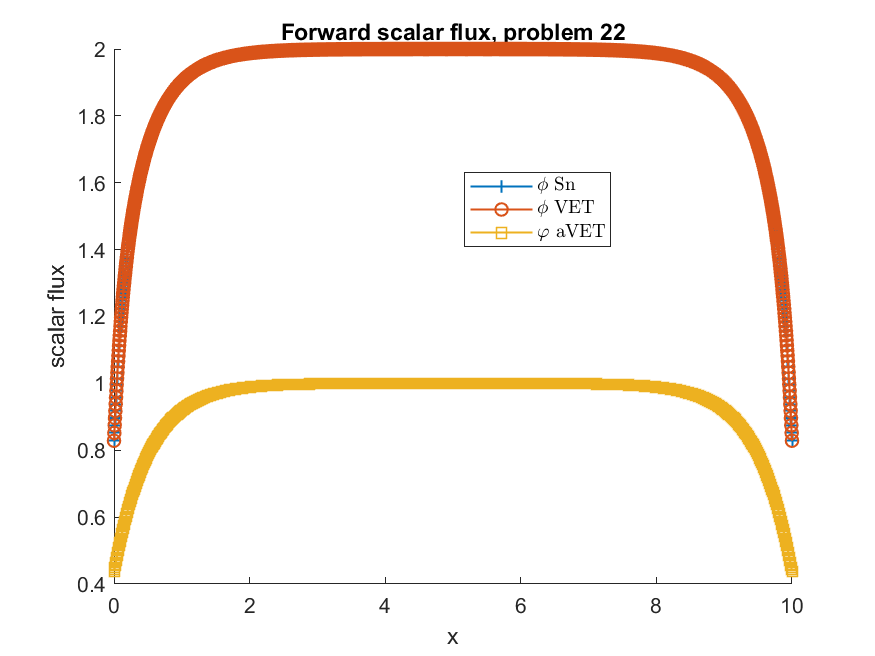
\includegraphics[width=.98\linewidth]{figures2/22phi.png}
%  \label{T1:sfig1}
%\end{subfigure}
%%
%\begin{subfigure}{0.45\textwidth}
%  \centering
%  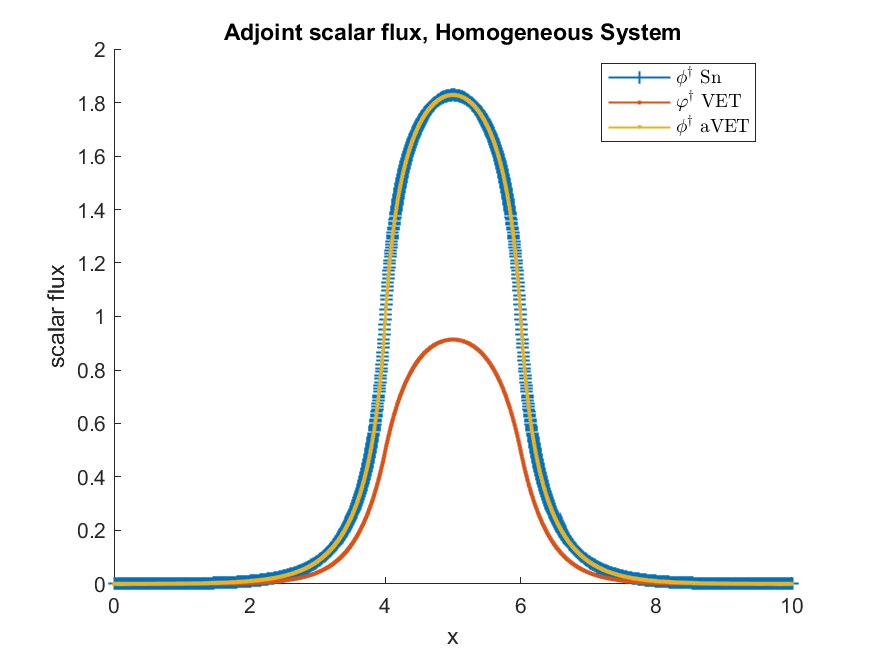
\includegraphics[width=.98\linewidth]{figures2/22phia.png}
%  \label{T1:sfig2}
%\end{subfigure}
%\end{figure}
%\end{frame}
%
% %%%%%%%%%%%%%%%%%%%%%%%%%%%%%%%%%%%%%%%%%%%%%%%%%%%%%%%%%%%%%%%%%%%%%%%%%%%%%%%%%%%%%%%%%%%%%%%%%%%%%%%%%%%
%
%\begin{frame}\frametitle{Homogeneous System, Homogeneous Perturbation}
% \begin{flushleft}
%
%\begin{figure}[H]
%\label{Trial1}
%\centering
%\begin{subfigure}{.5\textheight}
%  \centering
%  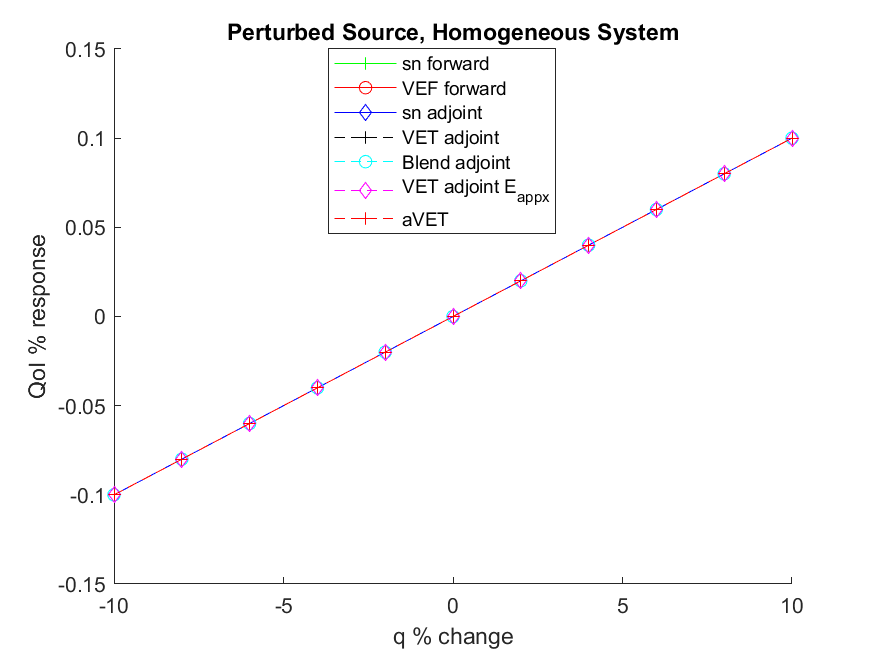
\includegraphics[width=.98\linewidth]{figures2/22qSens.png}
%  \label{T1:sfig1}
%\end{subfigure}%
%\begin{subfigure}{.5\textheight}
%  \centering
%  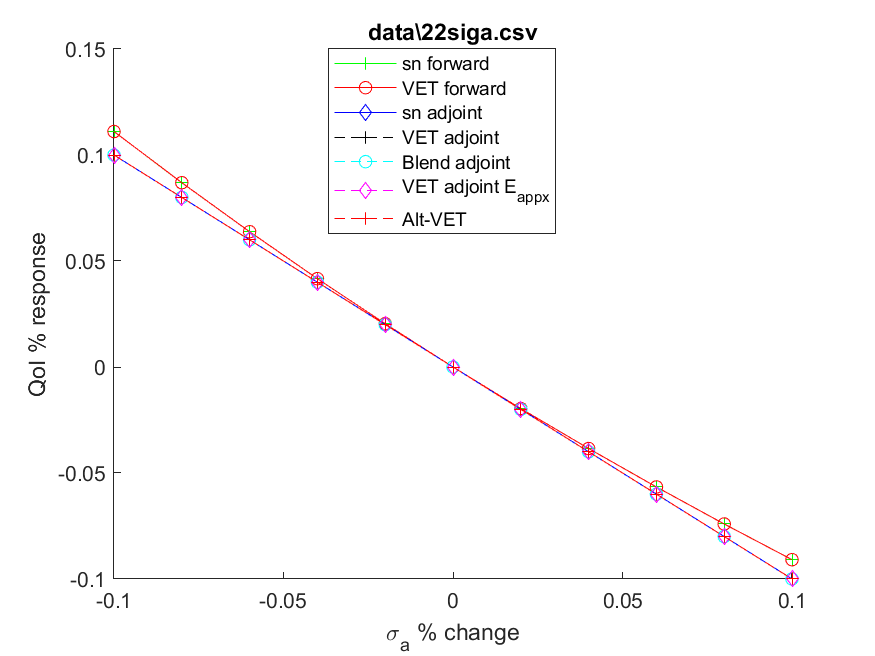
\includegraphics[width=.98\linewidth]{figures2/22sigaSens.png}
%  \label{T1:sfig2}
%\end{subfigure}
%%
%\begin{subfigure}{.5\textheight}
%  \centering
%  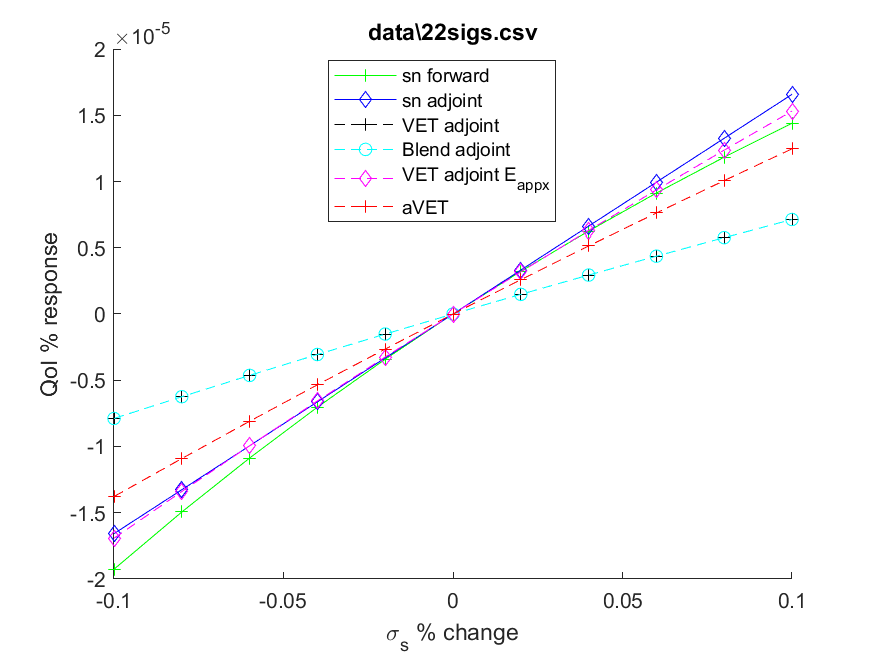
\includegraphics[width=.98\linewidth]{figures2/22sigsSens.png}
%  \label{T1:sfig3}
%\end{subfigure}%
%\begin{subfigure}{.5\textheight}
%  \centering
%  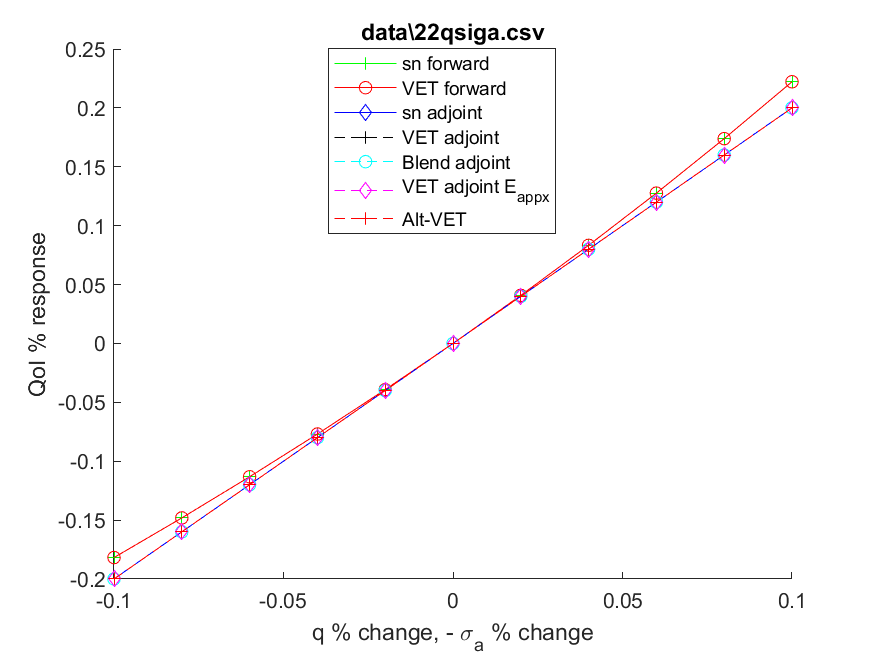
\includegraphics[width=.98\linewidth]{figures2/22qsigaSens.png}
%  \label{T1:sfig4}
%\end{subfigure}
%\end{figure}
%\end{flushleft}
%\end{frame}
%
% %%%%%%%%%%%%%%%%%%%%%%%%%%%%%%%%%%%%%%%%%%%%%%%%%%%%%%%%%%%%%%%%%%%%%%%%%%%%%%%%%%%%%%%%%%%%%%%%%%%%%%%%%%%
%
%\begin{frame}\frametitle{Homogeneous System, Homogeneous Perturbation}
%\begin{flushleft}
%\begin{itemize}
%\item Infinite medium approximation in both unperturbed and perturbed. $\phi_\infty=\frac{q}{\siga}$
%\item All methods exact for $q$ perturbations ($\delta \Edd \approx 0$ valid here).
%\item All adjoint methods show first-order approximation error for $\siga$ perturbations.
%\item Low sensitivity to $\sigs$ perturbations.
%\end{itemize}
%\end{flushleft}
%\end{frame}

 %%%%%%%%%%%%%%%%%%%%%%%%%%%%%%%%%%%%%%%%%%%%%%%%%%%%%%%%%%%%%%%%%%%%%%%%%%%%%%%%%%%%%%%%%%%%%%%%%%%%%%%%%%%

\begin{frame}\frametitle{Homogeneous System, Non-Homogeneous Perturbation}
        \begin{flushleft}
             Homogeneous System with Non-Homogeneous Perturbation
          	 \begin{itemize}
			      \item $\siga=1$, $\sigs=1$
			      \item $q=2$, $\psi^{\text{inc}}=0$
			      \item $\qoi = \int_4^6 \phi \, dx$. Means same adjoint flux as previous case.
			      \item \textcolor{red}{Perturbed for $0 \leq x \leq 6$}
  			 \end{itemize} 
            \end{flushleft}
\begin{figure}[H]
\label{Flux2}
\centering
\begin{subfigure}{0.45\textwidth}
  \centering
  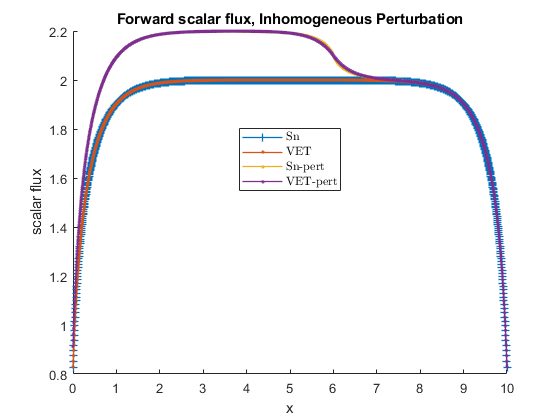
\includegraphics[width=.98\linewidth]{ANSfigures/23phip.png}
  \label{T1:sfig1}
\end{subfigure}
%
\begin{subfigure}{0.45\textwidth}
  \centering
  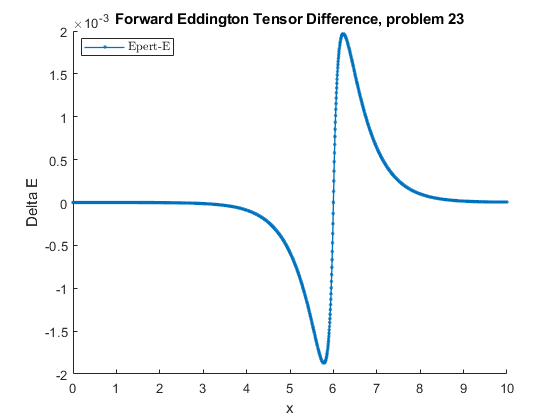
\includegraphics[width=.98\linewidth]{figures2/23deltaE.png}
  \label{T1:sfig2}
\end{subfigure}
\end{figure}
\end{frame}

 %%%%%%%%%%%%%%%%%%%%%%%%%%%%%%%%%%%%%%%%%%%%%%%%%%%%%%%%%%%%%%%%%%%%%%%%%%%%%%%%%%%%%%%%%%%%%%%%%%%%%%%%%%%

\begin{frame}\frametitle{Homogeneous System, Non-Homogeneous Perturbation}
 \begin{flushleft}

\begin{figure}[H]
\label{Trial2}
\begin{minipage}{.35\textwidth}
\centering
\begin{subfigure}{.45\textheight}
  \centering
  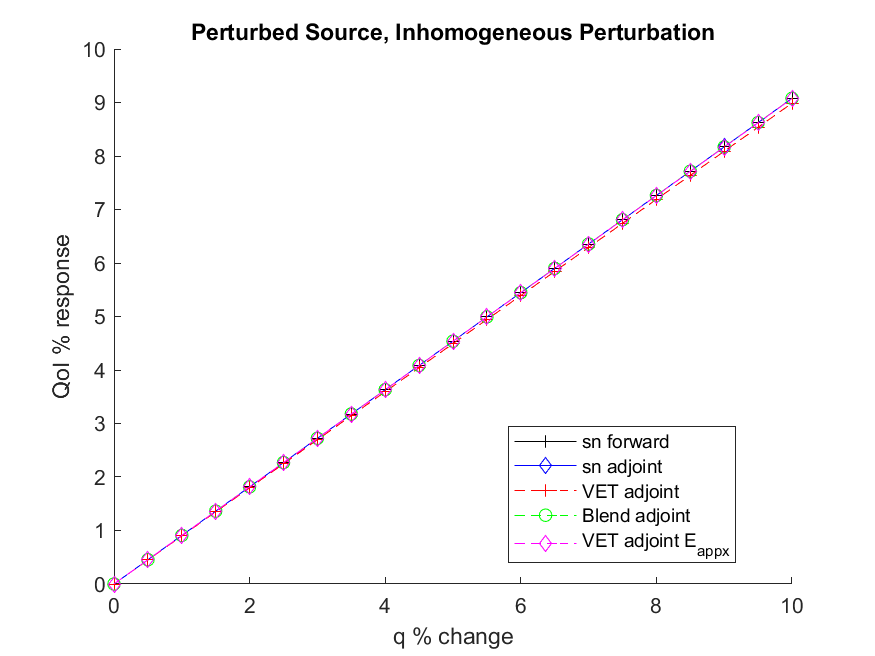
\includegraphics[width=.98\linewidth]{ANSfigures/23qSens.png}
  \label{T1:sfig1}
\end{subfigure}%

\begin{subfigure}{.45\textheight}
  \centering
  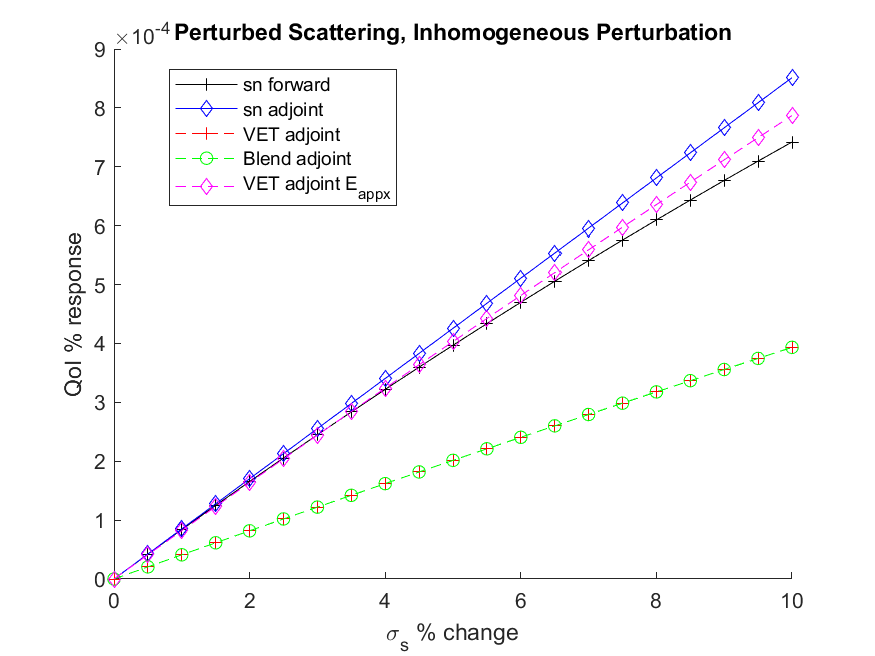
\includegraphics[width=.98\linewidth]{ANSfigures/23sigsSens.png}
\end{subfigure}
\end{minipage}
\begin{minipage}{.60\textwidth}
\begin{subfigure}{1\textwidth}
  \centering
  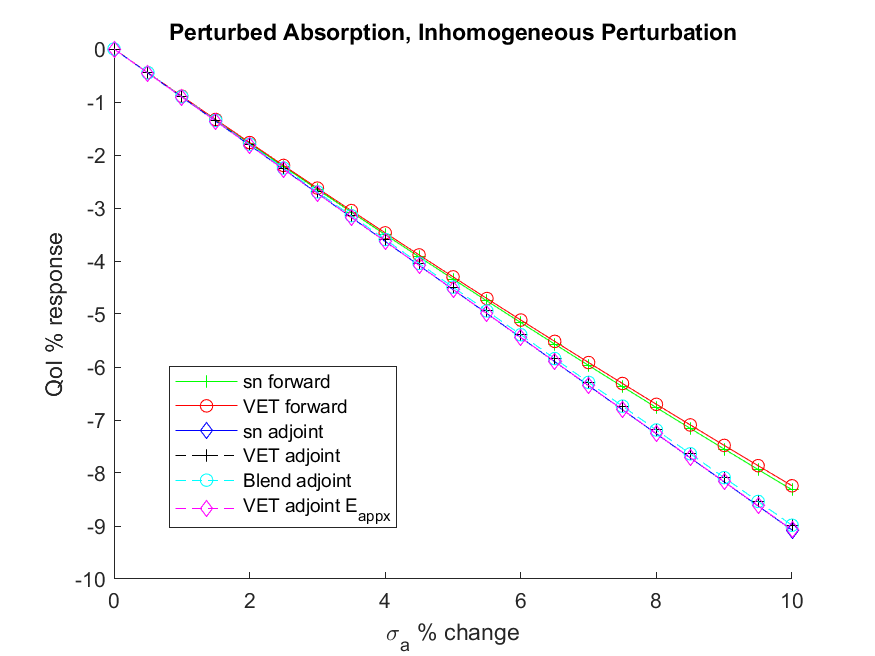
\includegraphics[width=.98\linewidth]{ANSfigures/23sigaSens.png}
\end{subfigure}%
%\begin{subfigure}{.5\textheight}
%  \centering
%  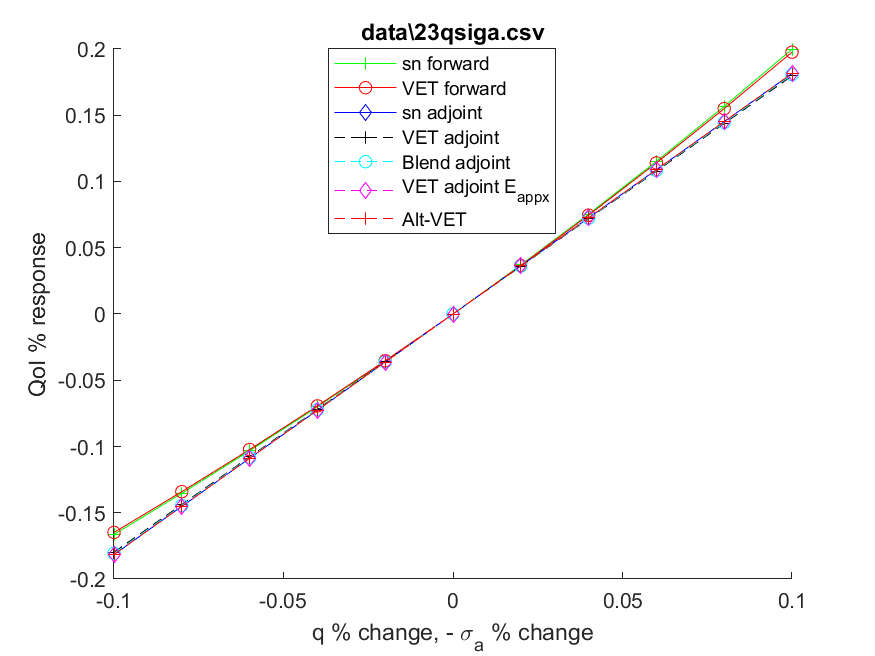
\includegraphics[width=.98\linewidth]{figures2/23qsigaSens.png}
%  \label{T1:sfig4}
%\end{subfigure}
\end{minipage}
\end{figure}
\end{flushleft}
\end{frame}

 %%%%%%%%%%%%%%%%%%%%%%%%%%%%%%%%%%%%%%%%%%%%%%%%%%%%%%%%%%%%%%%%%%%%%%%%%%%%%%%%%%%%%%%%%%%%%%%%%%%%%%%%%%%

\begin{frame}\frametitle{Homogeneous System, Non-Homogeneous Perturbation}
 \begin{flushleft}
\begin{itemize}
\item Infinite medium approximation in only unperturbed.
\item For source perturbations: Transport Adjdoint, blended, and aVET agree with transport forward.
\item For $\sigma$ perturbations, adjoint methods begin to show first order approximation error.
\item For $\sigma$ perturbations VET/blended adjoint are within $1 \%$ of transport adjoint. Eddington approximation and aVET nearly equal to transport adjoint $< 0.1 \%$ 
\item Still low sensitivity to $\sigs$ perturbations.
\end{itemize}
\end{flushleft}
\end{frame}

 %%%%%%%%%%%%%%%%%%%%%%%%%%%%%%%%%%%%%%%%%%%%%%%%%%%%%%%%%%%%%%%%%%%%%%%%%%%%%%%%%%%%%%%%%%%%%%%%%%%%%%%%%%%


%%%%%%%%%%%%%%%%%%%%%%%%%%%%%%%%%%%%%%%%%%%%%%%%%%%%%%%%%%%%%%%%%%%%%%%%%%%%%%%%%%%%%%%%%%%%%%%%%%%%%%%%%%%%
%
%\begin{frame}\frametitle{Reed Problem}
%        \begin{flushleft}
%             More complex Reed system
%          	 \begin{itemize}
%				\item $x \in [0,2), \quad \siga=50, \, 			\sigs=0, \, q=50, \, q^\dag=0 $\\
%				\item $x \in [2,3), \quad \siga=5, \, 			\sigs=0, \, q=0, \, q^\dag=0$ \\
%				\item $x \in [3,5), \quad \siga \approx 0, \,	\sigs=0, \, q=0, \, q^\dag=0$ \\
%				\item $x \in [5,6), \quad \siga=0.1, \, 		\sigs=0.9, \, q=1, \, q^\dag=0$ \\
%				\item $x \in [6,8], \quad \siga=0.1, \, 		\sigs=0.9, \, q=0, \, \tcr{q^\dag=1} $\\
%  			 \end{itemize} 
%            \end{flushleft}
%\begin{figure}[H]
%\label{Trial5}
%\centering
%\begin{subfigure}{0.45\textwidth}
%  \centering
%  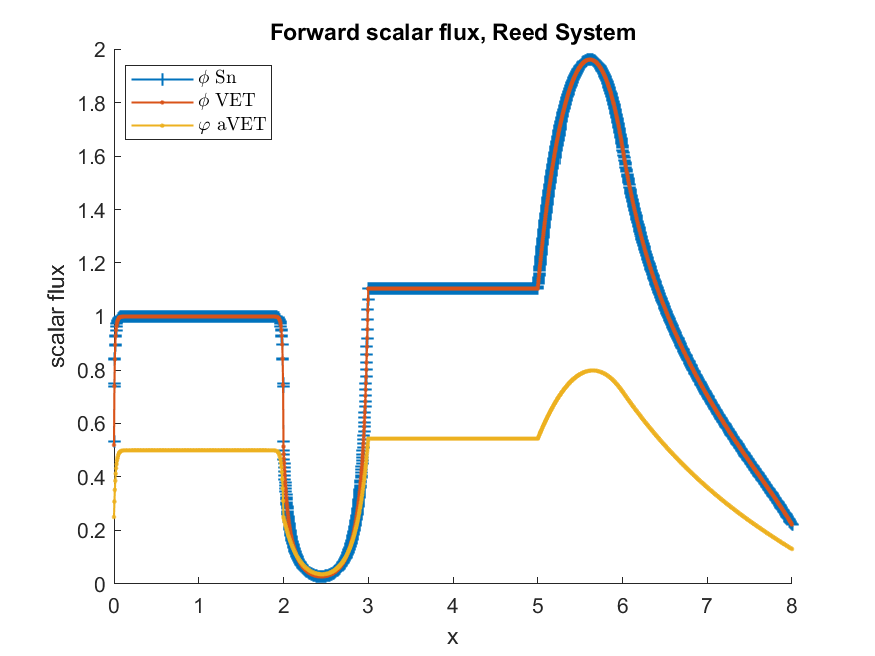
\includegraphics[width=.98\linewidth]{figures2/7phi.png}
%  \label{T1:sfig1}
%\end{subfigure}
%%
%\begin{subfigure}{0.45\textwidth}
%  \centering
%  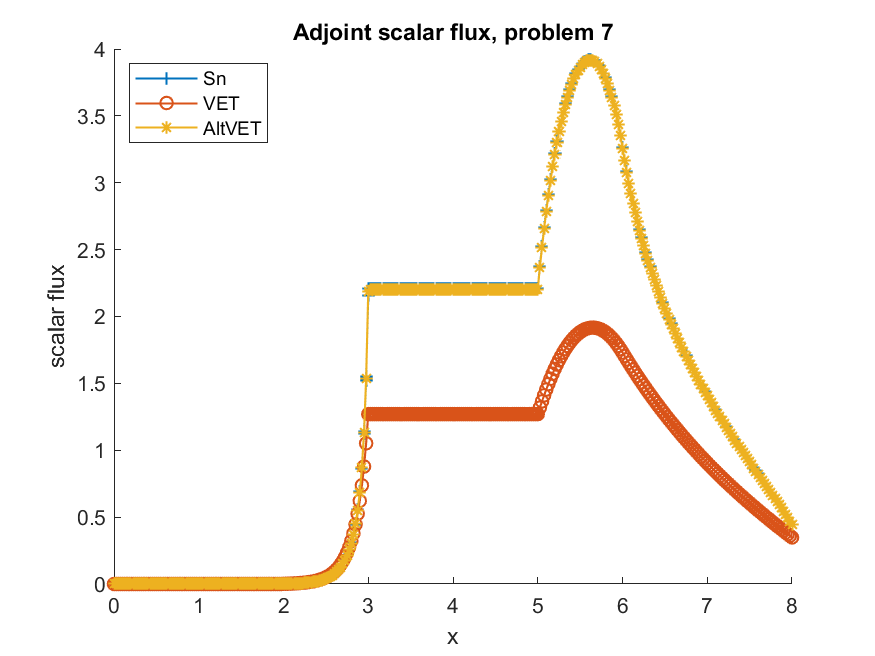
\includegraphics[width=.98\linewidth]{figures2/7phia.png}
%  \label{T1:sfig2}
%\end{subfigure}
%\end{figure}
%\end{frame}
%%%%%%%%%%%%%%%%%%%%%%%%%%%%%%%%%%%%%%%%%%%%%%%%%%%%%%%%%%%%%%%%%%%%%%%%%%%%%%%%%%%%%%%%%%%%%%%%%%%%%%%%%%%%
%\begin{frame}\frametitle{Reed Problem}
% \begin{flushleft}
%
%\begin{figure}[H]
%\label{Trial5}
%\centering
%\begin{subfigure}{.5\textheight}
%  \centering
%  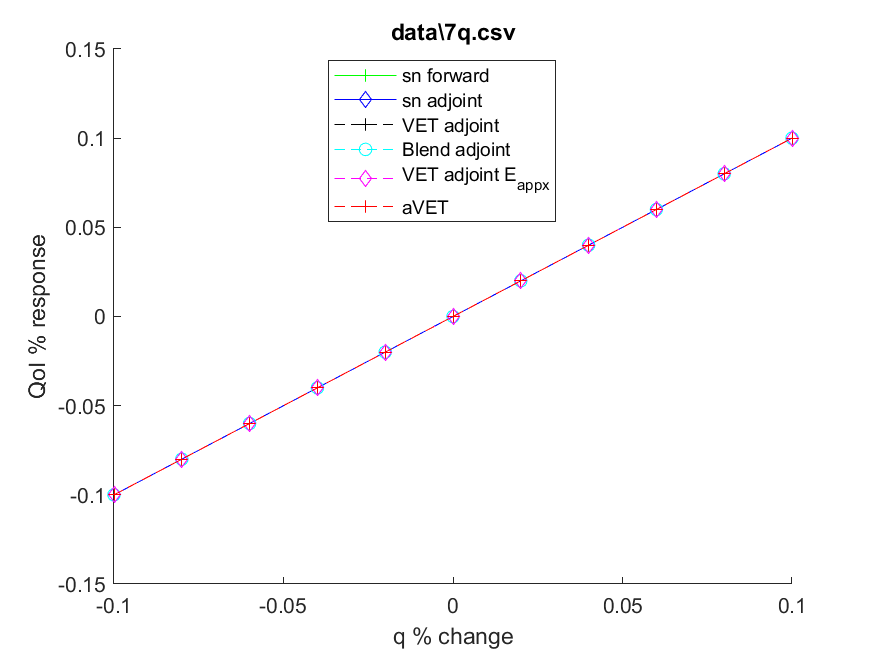
\includegraphics[width=.98\linewidth]{figures2/7qSens.png}
%  \label{T3:sfig1}
%\end{subfigure}%
%\begin{subfigure}{.5\textheight}
%  \centering
%  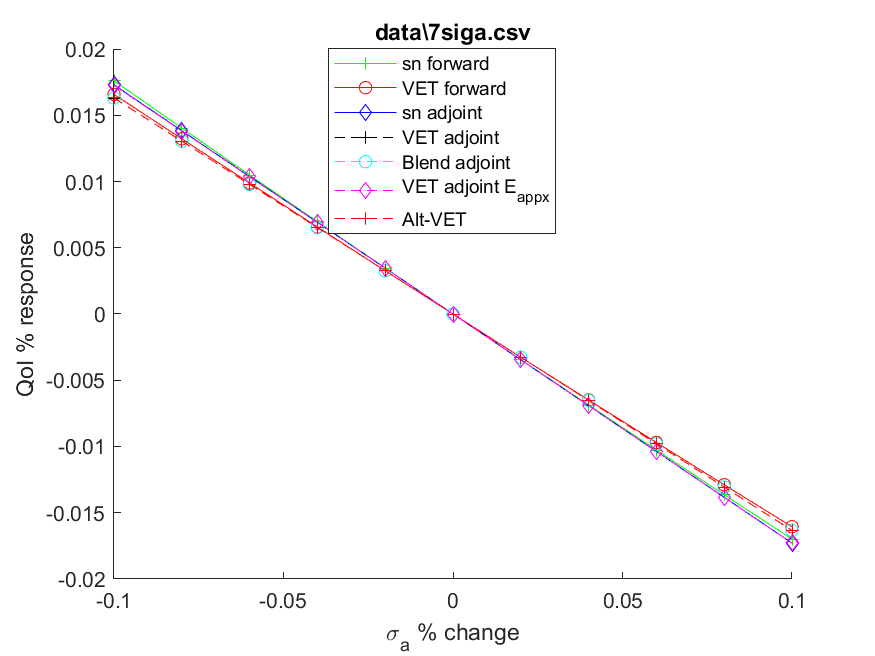
\includegraphics[width=.98\linewidth]{figures2/7sigaSens.png}
%  \label{T3:sfig2}
%\end{subfigure}
%%
%\begin{subfigure}{.5\textheight}
%  \centering
%  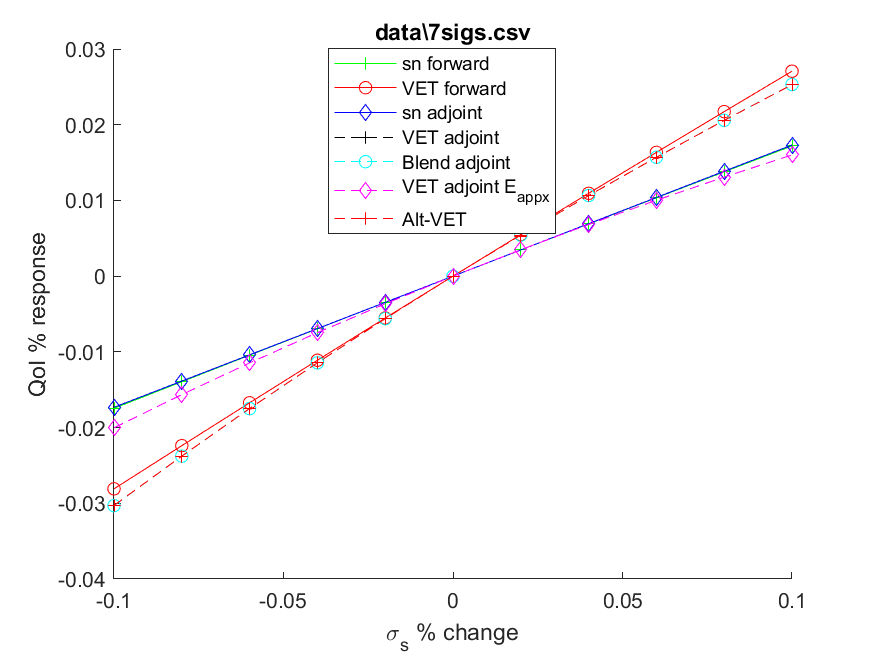
\includegraphics[width=.98\linewidth]{figures2/7sigsSens.png}
%  \label{T3:sfig3}
%\end{subfigure}%
%\begin{subfigure}{.5\textheight}
%  \centering
%  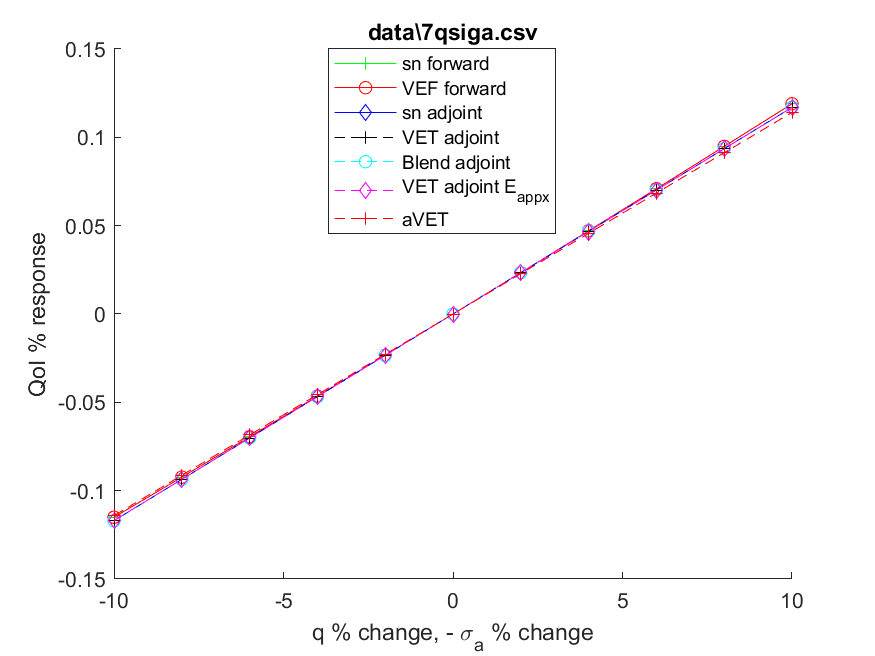
\includegraphics[width=.98\linewidth]{figures2/7qsigaSens.png}
%  \label{T3:sfig4}
%\end{subfigure}
%\end{figure}
%\end{flushleft}
%\end{frame}
%
%%%%%%%%%%%%%%%%%%%%%%%%%%%%%%%%%%%%%%%%%%%%%%%%%%%%%%%%%%%%%%%%%%%%%%%%%%%%%%%%%%%%%%%%%%%%%%%%%%%%%%%%%%%%
%
%\begin{frame}\frametitle{Reed Problem}
% \begin{flushleft}
%\begin{itemize}
%\item Source perturbations still behave as expected.
%\item Effect of $\delta \sigs$ more pronounced. VET forward, VET adjoint, blended, and aVET show deviations from transport methods. Eddington approximations reduces this. $\delta \Edd =0$ and $\delta \Edd^\dag=0$ approximation seemingly not valid here.
%\end{itemize}
%\end{flushleft}
%\end{frame}
%
%%%%%%%%%%%%%%%%%%%%%%%%%%%%%%%%%%%%%%%%%%%%%%%%%%%%%%%%%%%%%%%%%%%%%%%%%%%%%%%%%%%%%%%%%%%%%%%%%%%%%%%%%%%%
%%%%%%%%%%%%%%%%%%%%%%%%%%%%%%%%%%%%%%%%%%%%%%%%%%%%%%%%%%%%%%%%%%%%%%%%%%%%%%%%%%%%%%%%%%%%%%%%%%%%%%%%%%%%
%
%
%
%\begin{frame}\frametitle{Shielded Incident Isotropic Flux}
%        \begin{flushleft}
%             Shielded system with isotropic incident flux
%          	 \begin{itemize}
%			      \item Shield $\siga=0.5$, $\sigs=0.5$ for $1 \leq x  \leq 2$ (Vacuum else, $\sigt=10^{-8}$)
%			      \item $q=0$, $\psi^{\text{inc}}=1$ for $\mu > 0$; $0$ else
%			      \item $\qoi = \int_3^4 \phi \, dx$
%			      \item $\sigs$, $\siga$ perturbed in shield
%  			 \end{itemize} 
%            \end{flushleft}
%\begin{figure}[H]
%\label{Flux3}
%\centering
%\begin{subfigure}{0.45\textwidth}
%  \centering
%  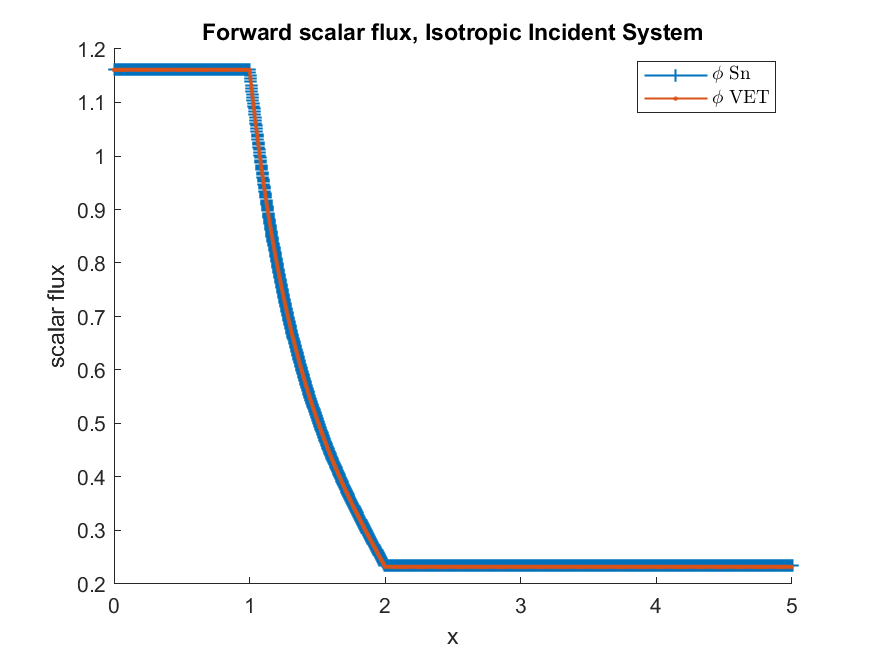
\includegraphics[width=.98\linewidth]{ANSfigures/24phi.png}
%  \label{T1:sfig1}
%\end{subfigure}
%%
%\begin{subfigure}{0.45\textwidth}
%  \centering
%  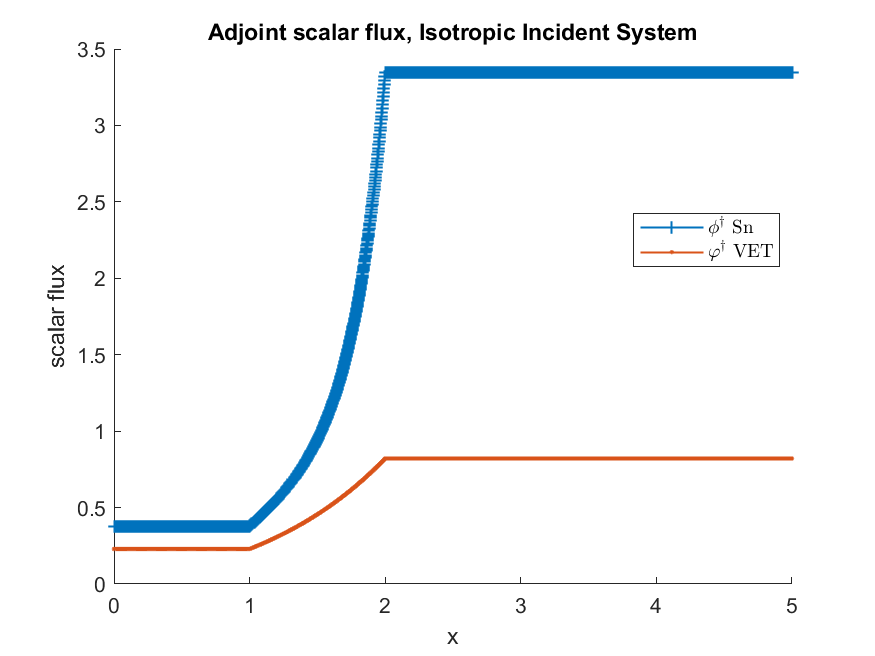
\includegraphics[width=.98\linewidth]{ANSfigures/24phia.png}
%  \label{T1:sfig2}
%\end{subfigure}
%\end{figure}
%\end{frame}
%
% %%%%%%%%%%%%%%%%%%%%%%%%%%%%%%%%%%%%%%%%%%%%%%%%%%%%%%%%%%%%%%%%%%%%%%%%%%%%%%%%%%%%%%%%%%%%%%%%%%%%%%%%%%%
%\begin{frame}\frametitle{Shielded Incident Isotropic Flux}
% \begin{flushleft}
%
%\begin{figure}[H]
%\label{Trial3}
%\begin{minipage}{.35\textwidth}
%\centering
%\begin{subfigure}{.45\textheight}
%  \centering
%  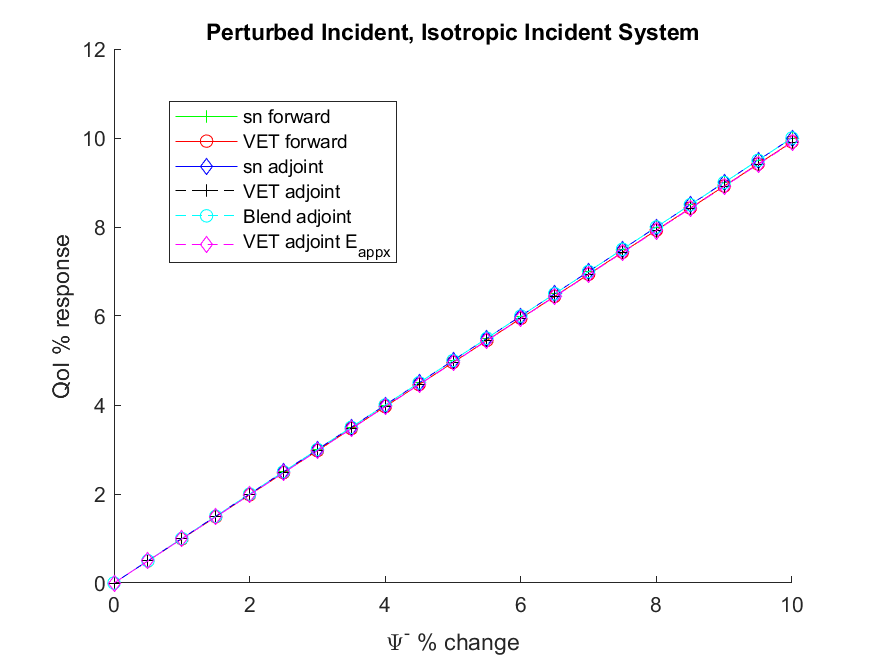
\includegraphics[width=.98\linewidth]{ANSfigures/24incSens.png}
%  \label{T1:sfig1}
%\end{subfigure}%
%
%\begin{subfigure}{.45\textheight}
%  \centering
%  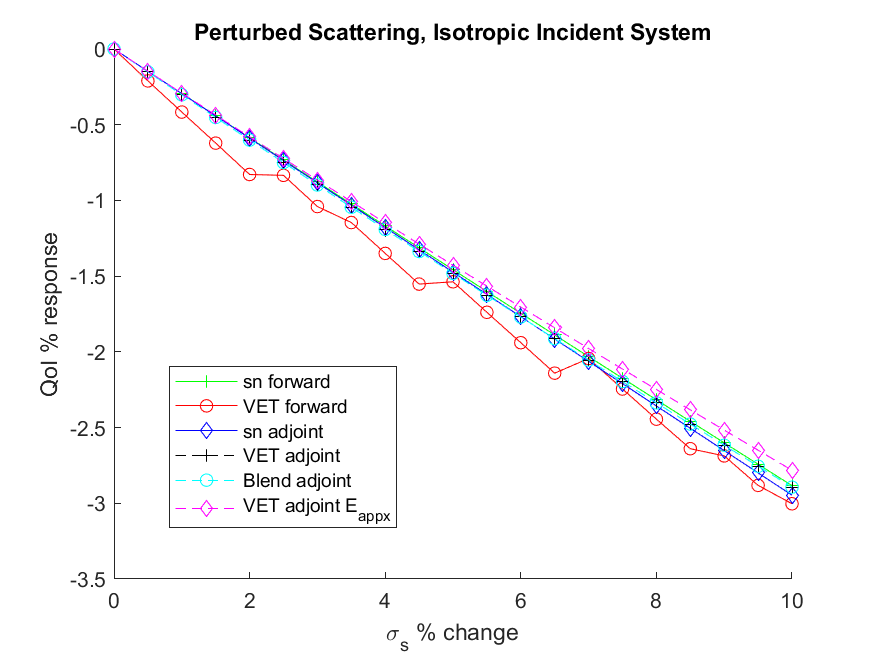
\includegraphics[width=.98\linewidth]{ANSfigures/24sigsSens.png}
%\end{subfigure}
%\end{minipage}
%\begin{minipage}{.60\textwidth}
%\begin{subfigure}{1\textwidth}
%  \centering
%  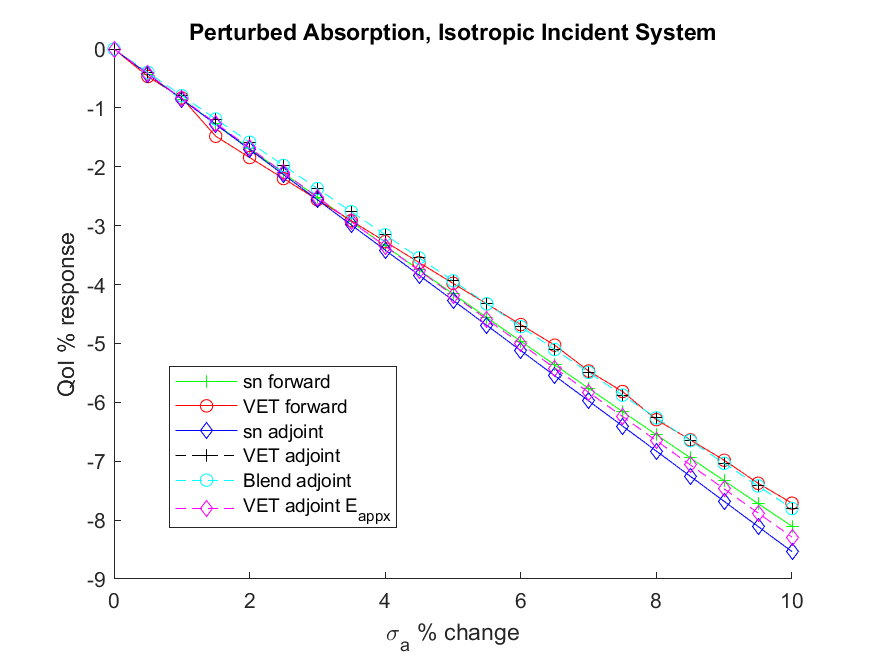
\includegraphics[width=.98\linewidth]{ANSfigures/24sigaSens.png}
%\end{subfigure}%
%%\begin{subfigure}{.5\textheight}
%%  \centering
%%  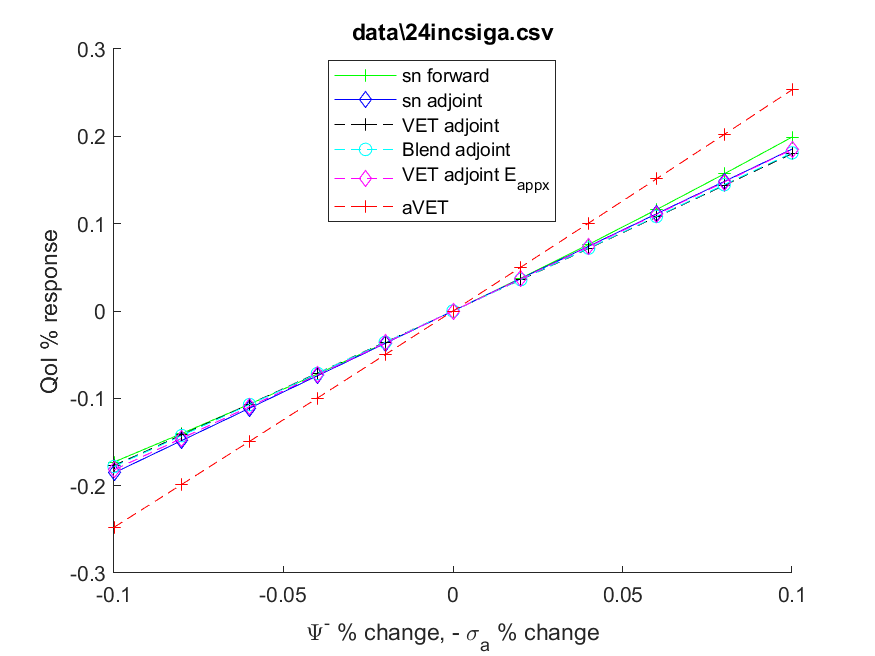
\includegraphics[width=.98\linewidth]{figures2/24incsigaSens.png}
%%  \label{T3:sfig4}
%%\end{subfigure}
%\end{minipage}
%\end{figure}
%\end{flushleft}
%\end{frame}
%
% %%%%%%%%%%%%%%%%%%%%%%%%%%%%%%%%%%%%%%%%%%%%%%%%%%%%%%%%%%%%%%%%%%%%%%%%%%%%%%%%%%%%%%%%%%%%%%%%%%%%%%%%%%%
%
%\begin{frame}\frametitle{Shielded Incident Isotropic Flux}
% \begin{flushleft}
%\begin{itemize}
%\item For incident flux perturbations: Transport Adjdoint, blended, and aVET agree with transport forward. Slight deviation in others.
%\item For source perturbations  VET adjoint shows minor deviations $\approx 1 \%$.
%\item About $5 \%$ error between VET adjoint and transport adjoint for $\delta \siga$. $\delta E$ approximation drops this to $0.5\%$.
%\item Somewhat stronger sensitivity to $\sigs$ perturbations, but still relatively weak.
%\item aVET appears to have strong deviations in this test for cross-section perturbations.
%\end{itemize}
%\end{flushleft}
%\end{frame}
%
%
%%%%%%%%%%%%%%%%%%%%%%%%%%%%%%%%%%%%%%%%%%%%%%%%%%%%%%%%%%%%%%%%%%%%%%%%%%%%%%%%%%%%%%%%%%%%%%%%%%%%%%%%%%%%
%
%\begin{frame}\frametitle{Shielded Incident Beam}
%        \begin{flushleft}
%             Shielded system with grazing incident beam $\mu=0.1834$
%          	 \begin{itemize}
%			      \item Shield $\siga=0.5$, $\sigs=0.5$ for $1 \leq x  \leq 2$ (Vacuum else, $\sigt=10^{-8}$)
%			      \item $q=0$, $\psi^{\text{inc}}=2.7571$ for $\mu=0.1834$ ($N=5$); $0$ else
%			      \item $\qoi = \int_3^4 \phi \, dx$
%			      \item $\sigs$, $\siga$ perturbed in shield
%  			 \end{itemize} 
%            \end{flushleft}
%\begin{figure}[H]
%\label{Flux4}
%\centering
%\begin{subfigure}{0.45\textwidth}
%  \centering
%  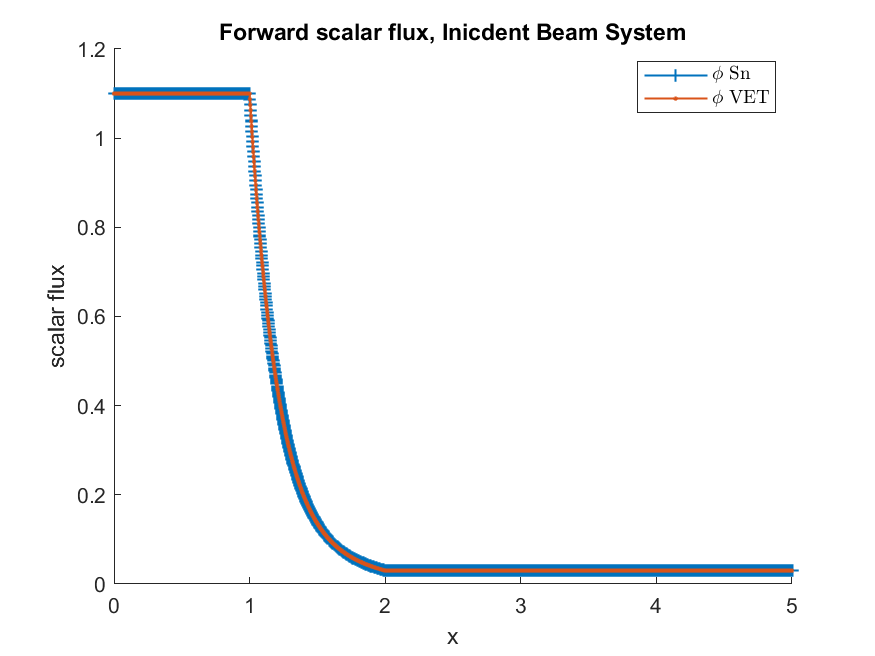
\includegraphics[width=.98\linewidth]{ANSfigures/25phi.png}
%  \label{T1:sfig1}
%\end{subfigure}
%%
%\begin{subfigure}{0.45\textwidth}
%  \centering
%  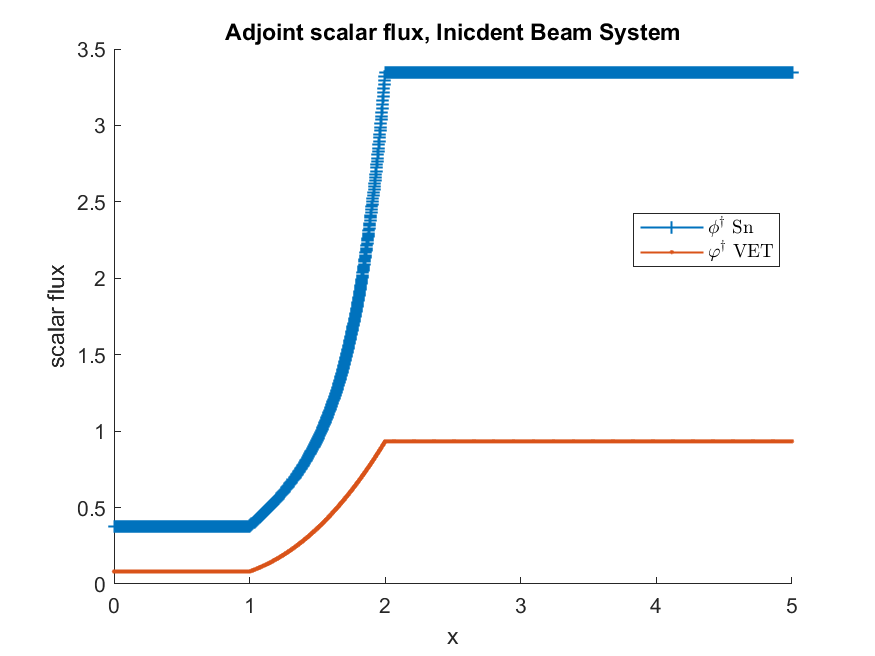
\includegraphics[width=.98\linewidth]{ANSfigures/25phia.png}
%  \label{T1:sfig2}
%\end{subfigure}
%\end{figure}
%\end{frame}
%
% %%%%%%%%%%%%%%%%%%%%%%%%%%%%%%%%%%%%%%%%%%%%%%%%%%%%%%%%%%%%%%%%%%%%%%%%%%%%%%%%%%%%%%%%%%%%%%%%%%%%%%%%%%%
%\begin{frame}\frametitle{Shielded Incident Beam}
% \begin{flushleft}
%
%\begin{figure}[H]
%\label{Trial4}
%\begin{minipage}{.35\textwidth}
%\centering
%\begin{subfigure}{.45\textheight}
%  \centering
%  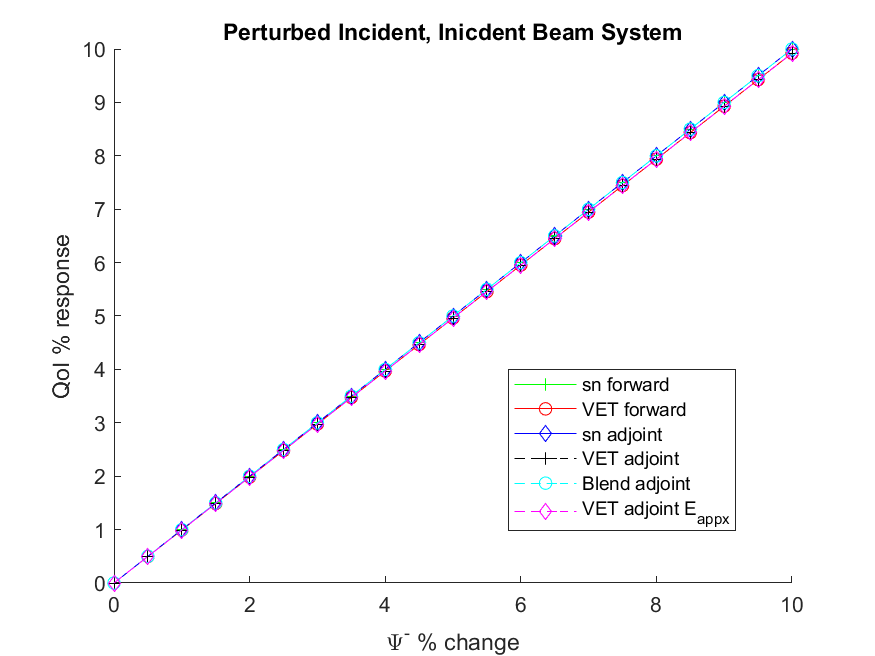
\includegraphics[width=.98\linewidth]{ANSfigures/25incSens.png}
%  \label{T1:sfig1}
%\end{subfigure}%
%
%\begin{subfigure}{.45\textheight}
%  \centering
%  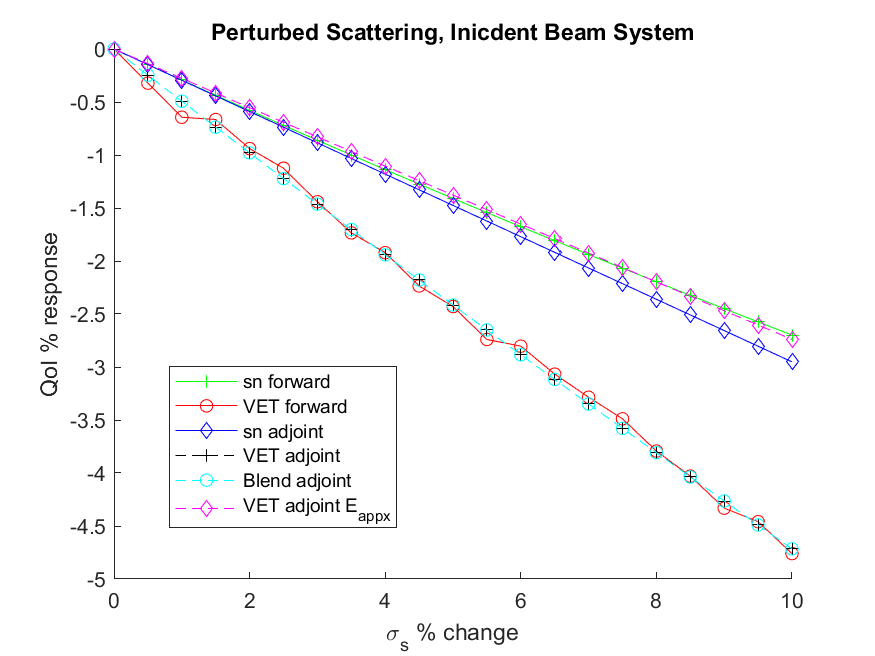
\includegraphics[width=.98\linewidth]{ANSfigures/25sigsSens.png}
%\end{subfigure}
%\end{minipage}
%\begin{minipage}{.60\textwidth}
%\begin{subfigure}{1\textwidth}
%  \centering
%  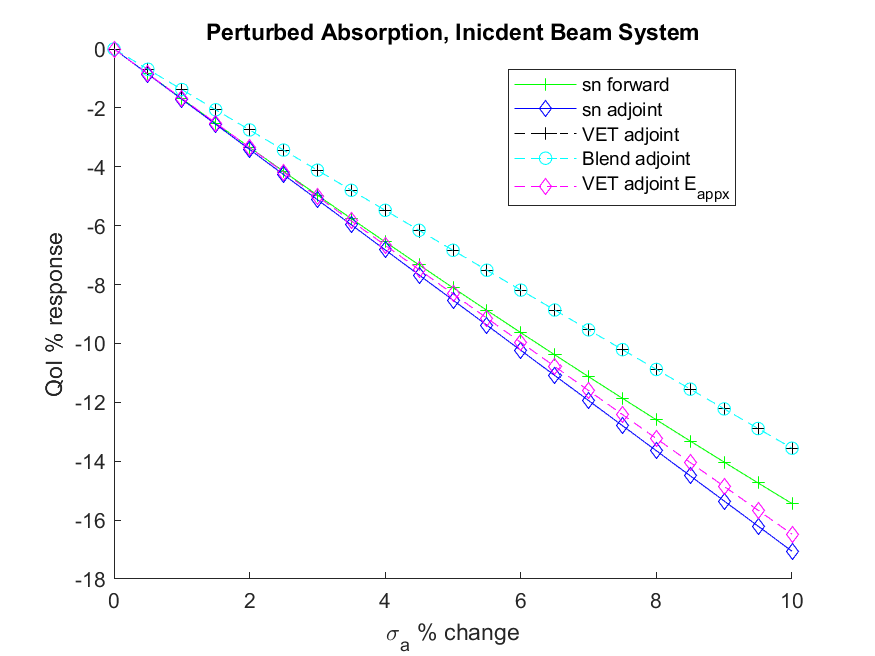
\includegraphics[width=.98\linewidth]{ANSfigures/25sigaSens.png}
%\end{subfigure}%
%%\begin{subfigure}{.5\textheight}
%%  \centering
%%  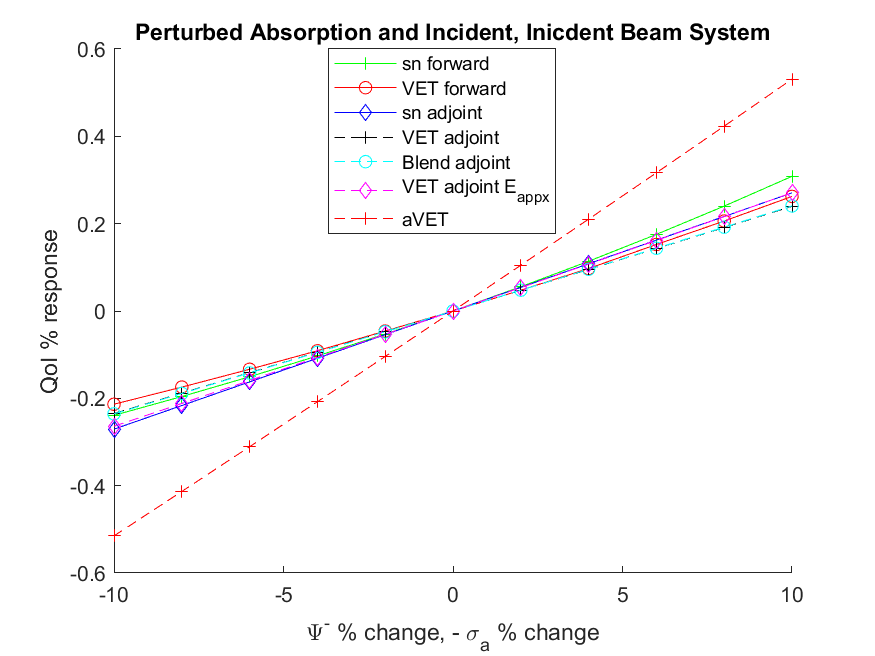
\includegraphics[width=.98\linewidth]{figures2/25incsigaSens.png}
%%\end{subfigure}
%\end{minipage}
%\end{figure}
%\end{flushleft}
%\end{frame}
%
%%%%%%%%%%%%%%%%%%%%%%%%%%%%%%%%%%%%%%%%%%%%%%%%%%%%%%%%%%%%%%%%%%%%%%%%%%%%%%%%%%%%%%%%%%%%%%%%%%%%%%%%%%%%
%
%\begin{frame}\frametitle{Shielded Incident Beam}
% \begin{flushleft}
%\begin{itemize}
%\item VET/blended method was worse for cross section perturbations, particularly scattering.
%\item $\delta \Edd$ approximation fared well and nearly reconciled transport adjoint and VET adjoint.
%\end{itemize}
%\end{flushleft}
%\end{frame}
%
% %%%%%%%%%%%%%%%%%%%%%%%%%%%%%%%%%%%%%%%%%%%%%%%%%%%%%%%%%%%%%%%%%%%%%%%%%%%%%%%%%%%%%%%%%%%%%%%%%%%%%%%%%%%
 
 
%%%%%%%%%%%%%%%%%%%%%%%%%%%%%%%%%%%%%%%%%%%%%%%%%%%%%%%%%%%%%%%%%%%%%%%%%%%%%%%%%%%%%%%%%%%%%%%%%%%%%%%%%%%

\begin{frame}\frametitle{Reed Problem: QoI comparison}
        \begin{flushleft}
             More complex Reed system\cite{buchan}. For this consider two separate QoI scenarios corresponding to \tcb{$q^\dag_1$} and \tcr{$q^\dag_2$}. We focus scattering perturbations.
          	 \begin{itemize}
				\item $x \in [0,2), \quad \siga=50, \, 			\sigs=0, \, q=50, \, q^\dag=0 $\\
				\item $x \in [2,3), \quad \siga=5, \, 			\sigs=0, \, q=0, \, q^\dag=0$ \\
				\item $x \in [3,5), \quad \siga \approx 0, \,	\sigs=0, \, q=0, \, \tcb{q^\dag_1=0}, \tcr{q^\dag_2=1}$, \\
				\item $x \in [5,6), \quad \siga=0.1, \, 		\sigs=0.9, \, q=1, \, q^\dag=0$ \\
				\item $x \in [6,8], \quad \siga=0.1, \, 		\sigs=0.9, \, q=0, \, \tcb{q^\dag_1=1}, \tcr{q^\dag_2=0} $
  			 \end{itemize} 
            \end{flushleft}
\begin{figure}[H]
\label{Trial5}
\centering
\begin{subfigure}{0.35\textwidth}
  \centering
  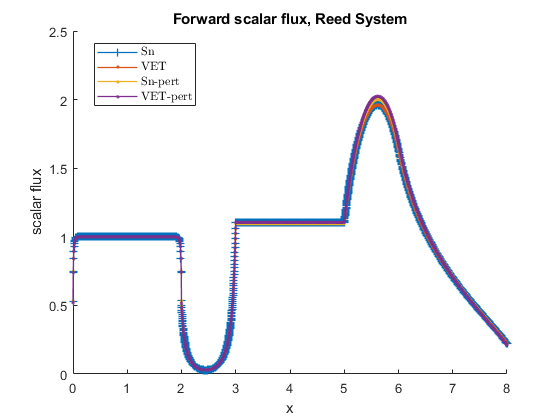
\includegraphics[width=.98\linewidth]{ANSfigures/7phip.png}
  \label{T1:sfig1}
\end{subfigure}
%
\begin{subfigure}{0.35\textwidth}
  \centering
  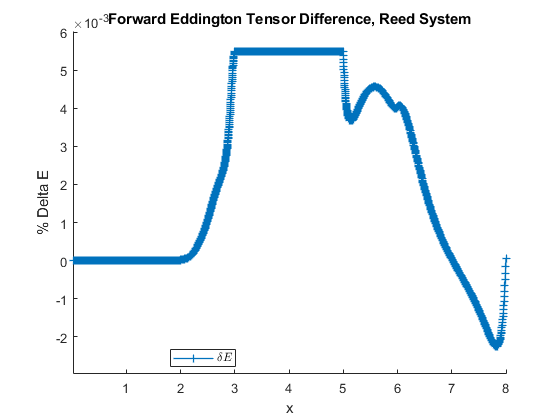
\includegraphics[width=.98\linewidth]{ANSfigures/7deltaE.png}
  \label{T1:sfig2}
\end{subfigure}
\end{figure}
\end{frame}
%%%%%%%%%%%%%%%%%%%%%%%%%%%%%%%%%%%%%%%%%%%%%%%%%%%%%%%%%%%%%%%%%%%%%%%%%%%%%%%%%%%%%%%%%%%%%%%%%%%%%%%%%%
\begin{frame}\frametitle{Reed Problem: QoI comparison}
 \begin{flushleft}

\begin{figure}[H]
\label{Trial5}
\centering
\begin{subfigure}{.5\textheight}
  \centering
  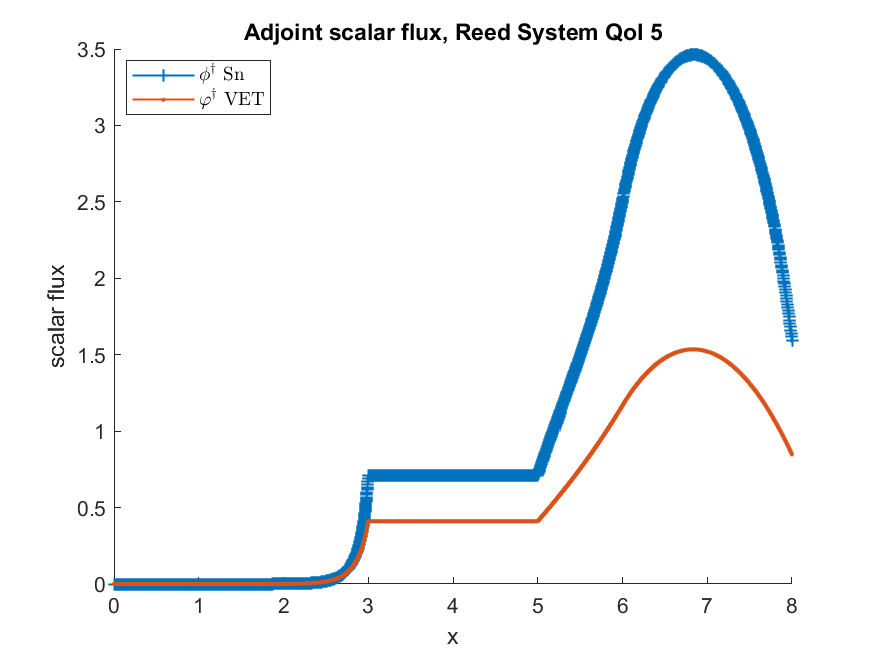
\includegraphics[width=.98\linewidth]{ANSfigures/774phia.png}
  \label{T3:sfig1}
\end{subfigure}%
\begin{subfigure}{.5\textheight}
  \centering
  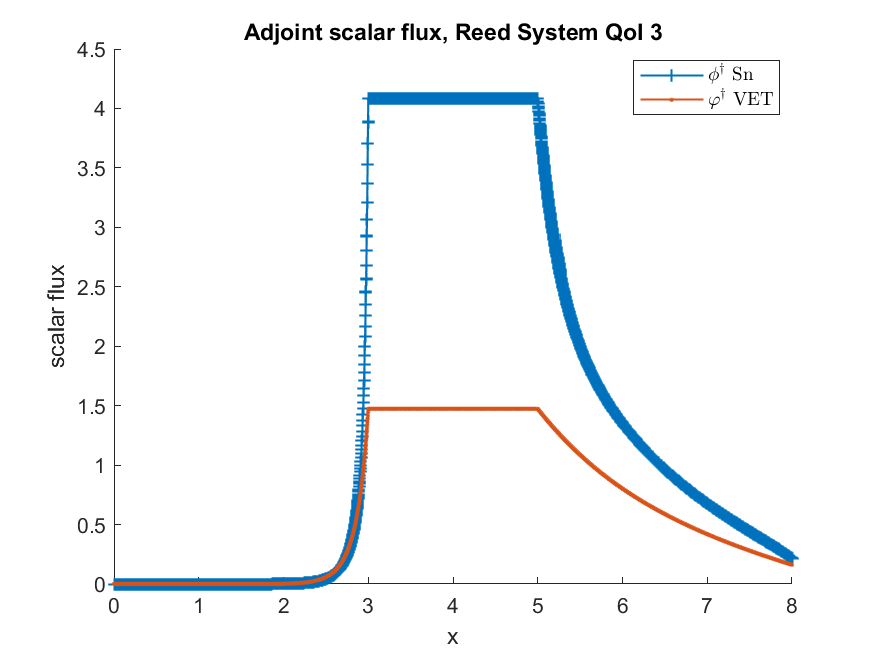
\includegraphics[width=.98\linewidth]{ANSfigures/772phia.png}
  \label{T3:sfig2}
\end{subfigure}
%
\begin{subfigure}{.5\textheight}
  \centering
  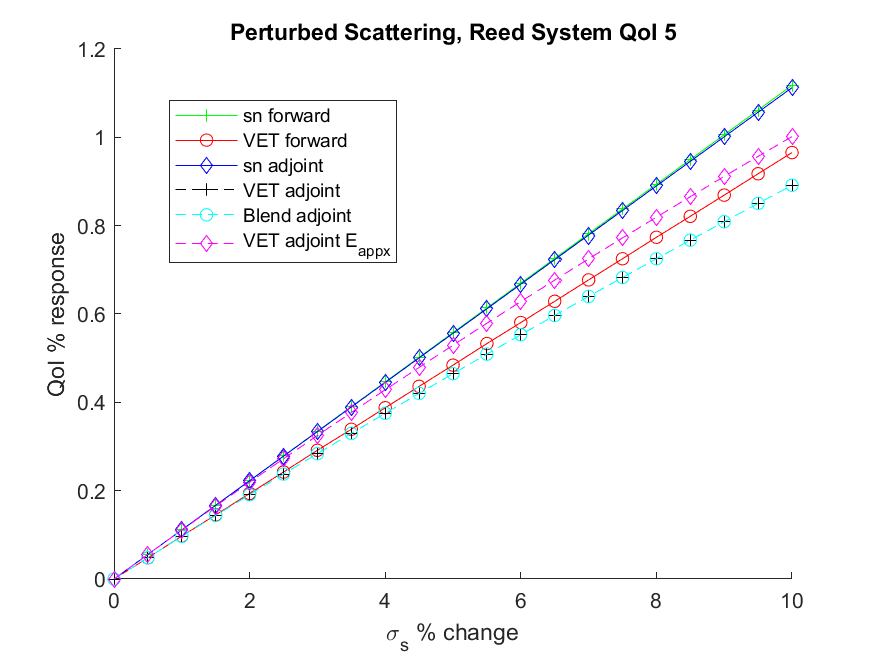
\includegraphics[width=.98\linewidth]{ANSfigures/774sigsSens.png}
  \label{T3:sfig3}
\end{subfigure}%
\begin{subfigure}{.5\textheight}
  \centering
  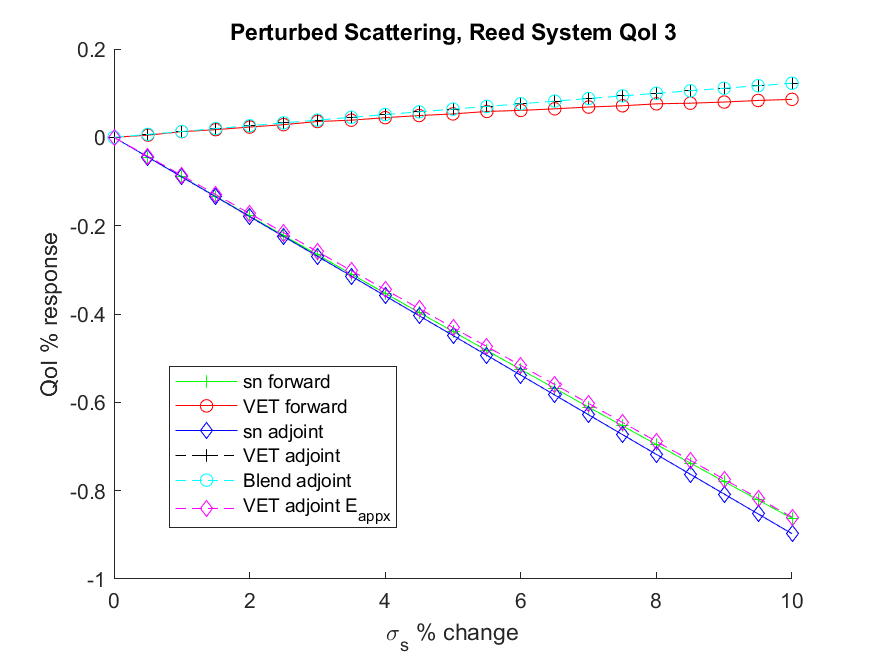
\includegraphics[width=.98\linewidth]{ANSfigures/772sigsSens.png}
  \label{T3:sfig4}
\end{subfigure}
\end{figure}
\end{flushleft}
\end{frame}

%%%%%%%%%%%%%%%%%%%%%%%%%%%%%%%%%%%%%%%%%%%%%%%%%%%%%%%%%%%%%%%%%%%%%%%%%%%%%%%%%%%%%%%%%%%%%%%%%%%%%%%%%%%

%%%%%%%%%%%%%%%%%%%%%%%%%%%%%%%%%%%%%%%%%%%%%%%%%%%%%%%%%%%%%%%%%%%%%%%%%%%%%%%%%%%%%%%%%%%%%%%%%%%%%%%%%%%

\begin{frame}\frametitle{Reed Problem: QoI comparison}
 \begin{flushleft}
\begin{itemize}
\item \qoi in scattering section fared fairly well for Eddington formulations, void \qoi did not
\vspace{2mm}
\item In void \qoi, the $\delta \Edd$ approximation method reconciled quite a bit of the error between VET and transport. Indicating there is a large contribution from $ - \bra  \isigt \div \left( \delta \Edd \phi \right),\tcr{ \grad \vefadj_2 }\ket$. Note that in the void $\isigt$ is large
\vspace{2mm} 
\item LHS of above product is the same for both scenarios, difference comes from behavior of $\tcr{ \grad \vefadj_2 }$
\end{itemize}
\end{flushleft}
\end{frame}

%%%%%%%%%%%%%%%%%%%%%%%%%%%%%%%%%%%%%%%%%%%%%%%%%%%%%%%%%%%%%%%%%%%%%%%%%%%%%%%%%%%%%%%%%%%%%%%%%%%%%%%%%%%

%%%%%%%%%%%%%%%%%%%%%%%%%%%%%%%%%%%%%%%%%%%%%%%%%%%%%%%%%%%%%%%%%%%%%%%%%%%%%%%%%%%%%%%%%%%%%%%%%%%%%%%%%%%
%\begin{frame}\frametitle{Reed Problem: QoI comparison term by term}
%\begin{flushleft}
%\begin{table}[H]
%\centering
%  \begin{tabular}{| l | r | r |}
%    \hline
%    Term  &  Right $q^\dag$ & Void  $q^\dag$\\ \hline
%    Unperturbed \qoi																	& 1.53202  & 2.21022 \\ \hline 
%     $+ \bra \delta \scalSource, \vefadj  \ket$											& 0 & 0\\ \hline
%     $- \bra \delta \siga \phi, \vefadj \ket$ 											& 0 & 0 \\ \hline
%     $- \bra \delta \isigt \div \left( \Edd \phi \right) , \grad \vefadj \ket$			& 0.0136565 & 0.00270713 \\ \hline
%     $+ \sbra \vefadj, 2 \delta J^{\text{inc}} \sket$										& 0 & 0\\ \hline
%     $- \bra  \isigt \div \left( \tcr{\delta \Edd} \phi \right), \grad \vefadj \ket$	& 0.00157771 & -0.0217348\\ \hline
%     $- \sbra \vefadj, \phi \tcr{\delta \BEdd} \sket$									& 0.000122458 & 2.3291e-05 \\ \hline
%    \end{tabular}
%  \caption{Term by Term comparison of VET method and $\delta \Edd$ approximation method for both the Reed QoI's under a $+10\%$ scattering perturbation.}
%\end{table}
%\end{flushleft}
%\end{frame}
%%%%%%%%%%%%%%%%%%%%%%%%%%%%%%%%%%%%%%%%%%%%%%%%%%%%%%%%%%%%%%%%%%%%%%%%%%%%%%%%%%%%%%%%%%%%%%%%%%%%%%%%%%%

%%%%%%%%%%%%%%%%%%%%%%%%%%%%%%%%%%%%%%%%%%%%%%%%%%%%%%%%%%%%%%%%%%%%%%%%%%%%%%%%%%%%%%%%%%%%%%%%%%%%%%%%%%%
\section{Wrap Up}	% define sections here, it is possible to get section slides automatically, but this is not enabled
\subsection{}	% we have to keep these to get the navigation
%%%%%%%%%%%%%%%%%%%%%%%%%%%%%%%%%%%%%%%%%%%%%%%%%%%%%%%%%%%%%%%%%%%%%%%%%%%%%%%%%%%%%%%%%%%%%%%%%%%%%%%%%%%
 %%%%%%%%%%%%%%%%%%%%%%%%%%%%%%%%%%%%%%%%%%%%%%%%%%%%%%%%%%%%%%%%%%%%%%%%%%%%%%%%%%%%%%%%%%%%%%%%%%%%%%%%%%%

\begin{frame}\frametitle{Takeaways}
\begin{flushleft}
\begin{itemize}
\item The 3 VET formulations show ability to approximate $\delta \qoi$ in many of the test cases, response function in void shows issues for cross-section perturbations. 
\vspace{2mm}
\item Blended method may offer a quick refinement over the straightforward VET, at the expense of an additional SN solve to get transport adjoint.
\vspace{2mm}
\item $\delta \Edd$ method appears to work quite well, but requires additional SN solves to parameterize the perturbation space. 


\end{itemize}
\end{flushleft}
\end{frame}

\begin{frame}\frametitle{Looking Forward}
\begin{flushleft}
\begin{itemize}
\item Extend tests to 2D/3D. Strong sensitivity to $\sigs$ is difficult to test in the 1D system. Inability to scatter ``around'' obstacles.
\vspace{2mm}
\item Potentially extend $\delta \Edd$ method to the aVET formulation.
\vspace{2mm}
\item Focus on streaming/void problems.
\end{itemize}
\end{flushleft}
\end{frame}

\begin{frame}\frametitle{References}
\begin{flushleft}
\bibliography{QoI_MS} 
\bibliographystyle{ieeetr}
\end{flushleft}
\end{frame}

\begin{frame}\frametitle{Acknowledgments}
\begin{flushleft}
\begin{itemize}
%\item Would like to thank my advisor Professor Jean C. Ragusa for invaluable help and heading my defense committee
%\item Also extend thanks to my defense committee members Professor Marvin L. Adams and Bojan Popov  
\item The work presented was supported by a graduate assistantship from the U.S. DOE NNSA's PSAAP program (Predictive Science Academic Alliance Program), Grant DE-NA0002376.  
\end{itemize}
\end{flushleft}
\end{frame}


%%%%%%%%%%%%%%%%%%%%%%%%%%%%%%%%%%%%%%%%%%%%%%%%%%%%%%%%%%%%%%%%%%%%%%%%%%%%%%%%%%%%%%%%%%%%%%%%%%%%%%%%%%%
\appendix
\newcounter{finalframe}
\setcounter{finalframe}{\value{framenumber}}
\section{Additional Slides}	% define sections here, it is possible to get section slides automatically, but this is not enabled
\subsection{}	% we have to keep these to get the navigation
%%%%%%%%%%%%%%%%%%%%%%%%%%%%%%%%%%%%%%%%%%%%%%%%%%%%%%%%%%%%%%%%%

%%%%%%%%%%%%%%%%%%%%%%%%%%%%%%%%%%%%%%%%%%%%%%%%%%%%%%%%%%%%%%%%%%%%%%%%%%%%%%%%%%%%%%%%%%%%%%%%%%%%%%%%%%%
\begin{frame}\frametitle{Appendix: VET Boundary Condition Derivation}
 \begin{flushleft}
\begin{equation}
\begin{split}
2 J^{\text{inc}}(\vr) 
&\equiv  2 \int_{\vO \cdot \vn <0 }  d \Omega\, | \vO \cdot \vec{n} | \psi^{\text{inc}}(\vr,\vO) \\
&= 2\int_{\vO \cdot \vn <0 } d \Omega\,  | \vO \cdot \vn |  \psi(\vr,\vO)\\
&= \int_{4\pi} d \Omega\,  \left( | \vO \cdot \vn |- \vO\cdot\vn\right)  \psi(\vr,\vO) \\
&= \BEdd(\vr) \phi(\vr) - \vn \cdot \textcolor{red}{\vJ} \\
&= \BEdd \phi + \vn \cdot \frac{1}{\sigt} \div \Edd \phi 
\end{split}
\end{equation}
\end{flushleft}
\end{frame}
%%%%%%%%%%%%%%%%%%%%%%%%%%%%%%%%%%%%%%%%%%%%%%%%%%%%%%%%%%%%%%%%%%%%%%%%%%%%%%%%%%%%%%%%%%%%%%%%%%%%%%%%%%%

 %%%%%%%%%%%%%%%%%%%%%%%%%%%%%%%%%%%%%%%%%%%%%%%%%%%%%%%%%%%%%%%%%%%%%%%%%%%%%%%%%%%%%%%%%%%%%%%%%%%%%%%%%%%

\begin{frame}\frametitle{Shielded Incident Isotropic Flux}
        \begin{flushleft}
             Shielded system with isotropic incident flux
          	 \begin{itemize}
			      \item Shield $\siga=0.5$, $\sigs=0.5$ for $1 \leq x  \leq 2$ (Vacuum else, $\sigt=10^{-8}$)
			      \item $q=0$, $\psi^{\text{inc}}=1$ for $\mu > 0$; $0$ else
			      \item $\qoi = \int_3^4 \phi \, dx$
			      \item $\sigs$, $\siga$ perturbed in shield
  			 \end{itemize} 
            \end{flushleft}
\begin{figure}[H]
\label{Flux3}
\centering
\begin{subfigure}{0.45\textwidth}
  \centering
  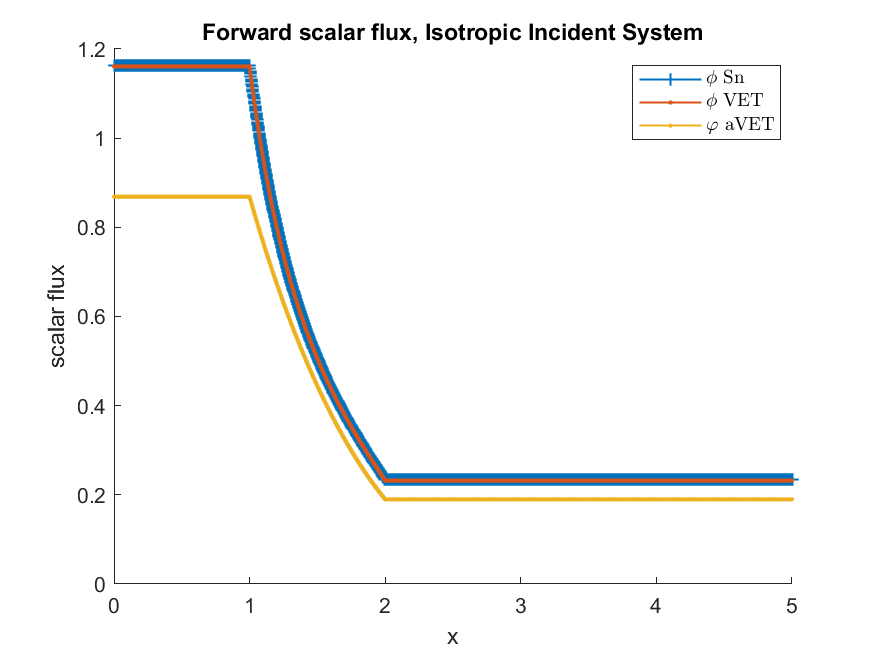
\includegraphics[width=.98\linewidth]{figures2/24phi.png}
  \label{T1:sfig1}
\end{subfigure}
%
\begin{subfigure}{0.45\textwidth}
  \centering
  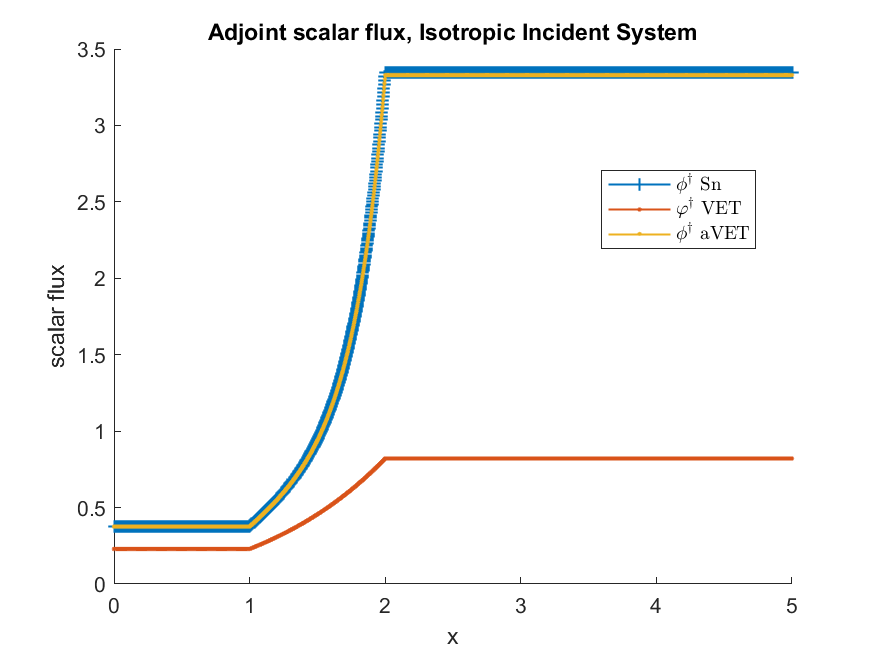
\includegraphics[width=.98\linewidth]{figures2/24phia.png}
  \label{T1:sfig2}
\end{subfigure}
\end{figure}
\end{frame}

 %%%%%%%%%%%%%%%%%%%%%%%%%%%%%%%%%%%%%%%%%%%%%%%%%%%%%%%%%%%%%%%%%%%%%%%%%%%%%%%%%%%%%%%%%%%%%%%%%%%%%%%%%%%
\begin{frame}\frametitle{Shielded Incident Isotropic Flux}
 \begin{flushleft}

\begin{figure}[H]
\label{Trial3}
\begin{minipage}{.35\textwidth}
\centering
\begin{subfigure}{.45\textheight}
  \centering
  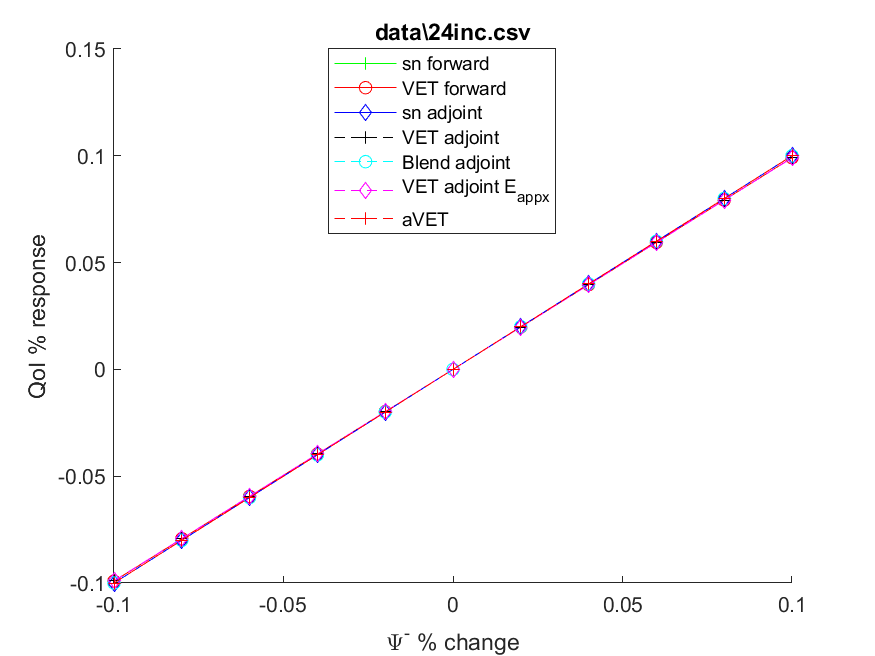
\includegraphics[width=.98\linewidth]{figures2/24incSens.png}
  \label{T1:sfig1}
\end{subfigure}%

\begin{subfigure}{.45\textheight}
  \centering
  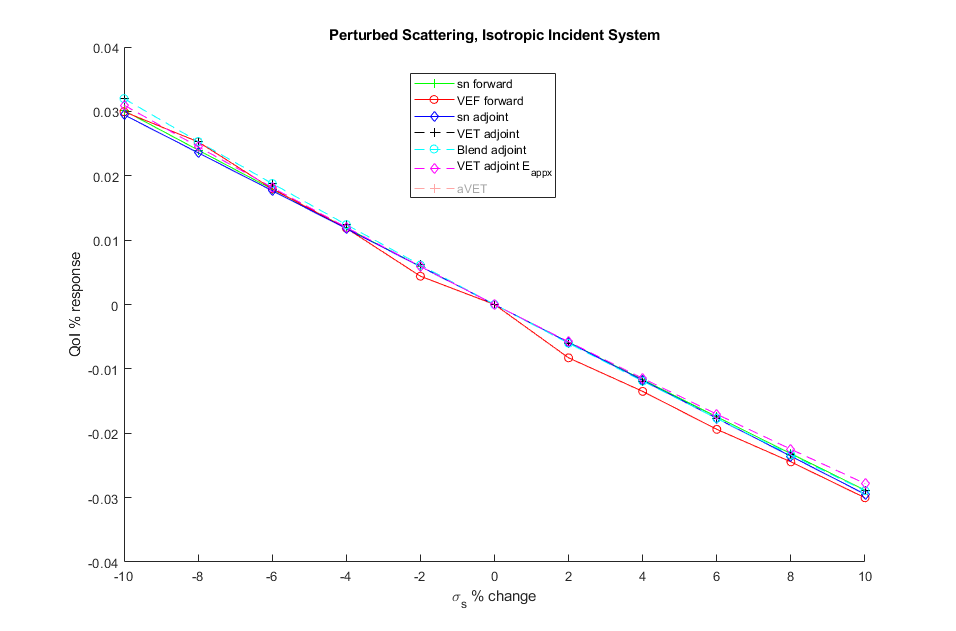
\includegraphics[width=.98\linewidth]{figures2/24sigsSensNoavet.png}
\end{subfigure}
\end{minipage}
\begin{minipage}{.60\textwidth}
\begin{subfigure}{1\textwidth}
  \centering
  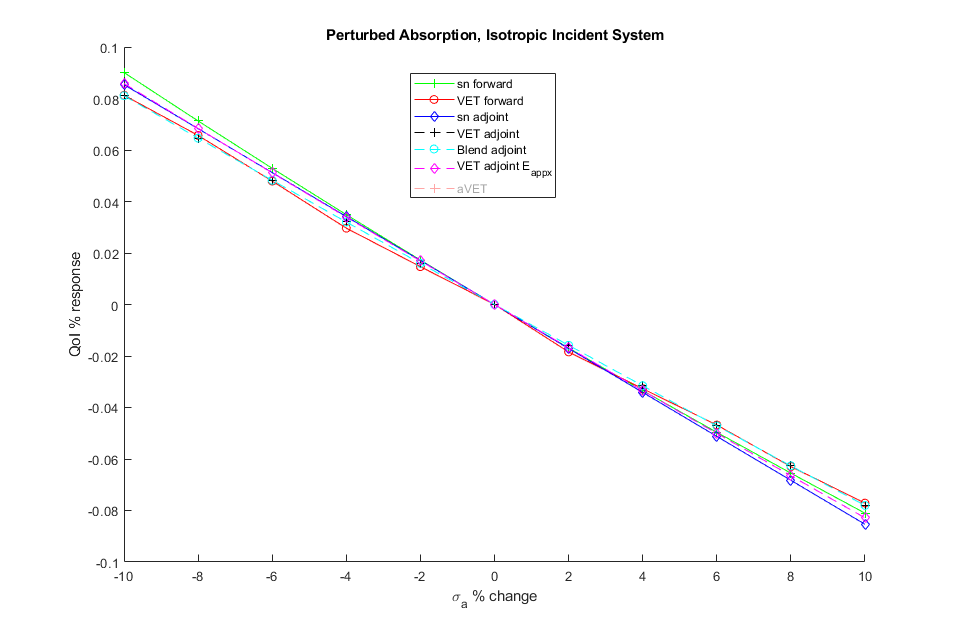
\includegraphics[width=.98\linewidth]{figures2/24sigaSensNoavet.png}
\end{subfigure}%
%\begin{subfigure}{.5\textheight}
%  \centering
%  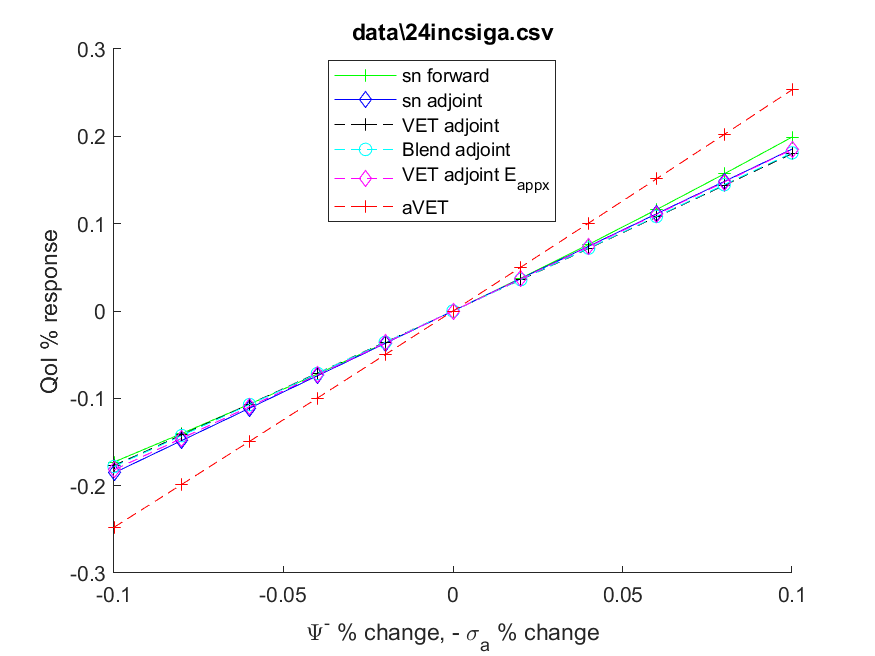
\includegraphics[width=.98\linewidth]{figures2/24incsigaSens.png}
%  \label{T3:sfig4}
%\end{subfigure}
\end{minipage}
\end{figure}
\end{flushleft}
\end{frame}

 %%%%%%%%%%%%%%%%%%%%%%%%%%%%%%%%%%%%%%%%%%%%%%%%%%%%%%%%%%%%%%%%%%%%%%%%%%%%%%%%%%%%%%%%%%%%%%%%%%%%%%%%%%%

\begin{frame}\frametitle{Shielded Incident Isotropic Flux}
 \begin{flushleft}
\begin{itemize}
\item For incident flux perturbations: Transport Adjdoint, blended, and aVET agree with transport forward. Slight deviation in others.
\item For source perturbations  VET adjoint shows minor deviations $\approx 1 \%$.
\item About $5 \%$ error between VET adjoint and transport adjoint for $\delta \siga$. $\delta E$ approximation drops this to $0.5\%$.
\item Somewhat stronger sensitivity to $\sigs$ perturbations, but still relatively weak.
\item aVET appears to have strong deviations in this test for cross-section perturbations.
\end{itemize}
\end{flushleft}
\end{frame}

 %%%%%%%%%%%%%%%%%%%%%%%%%%%%%%%%%%%%%%%%%%%%%%%%%%%%%%%%%%%%%%%%%%%%%%%%%%%%%%%%%%%%%%%%%%%%%%%%%%%%%%%%%%%

%%%%%%%%%%%%%%%%%%%%%%%%%%%%%%%%%%%%%%%%%%%%%%%%%%%%%%%%%%%%%%%%%%%%%%%%%%%%%%%%%%%%%%%%%%%%%%%%%%%%%%%%%%%
%%%%%%%%%%%%%%%%%%%%%%%%%%%%%%%%%%%%%%%%%%%%%%%%%%%%%%%%%%%%%%%%%%%%%%%%%%%%%%%%%%%%%%%%%%%%%%%%%%%%%%%%%%%

\begin{frame}\frametitle{Shielded Incident Beam}
        \begin{flushleft}
             Shielded system with grazing incident beam $\mu=0.1834$
          	 \begin{itemize}
			      \item Shield $\siga=0.5$, $\sigs=0.5$ for $1 \leq x  \leq 2$ (Vacuum else, $\sigt=10^{-8}$)
			      \item $q=0$, $\psi^{\text{inc}}=2.7571$ for $\mu=0.1834$ ($N=5$); $0$ else
			      \item $\qoi = \int_3^4 \phi \, dx$
			      \item $\sigs$, $\siga$ perturbed in shield
  			 \end{itemize} 
            \end{flushleft}
\begin{figure}[H]
\label{Flux4}
\centering
\begin{subfigure}{0.45\textwidth}
  \centering
  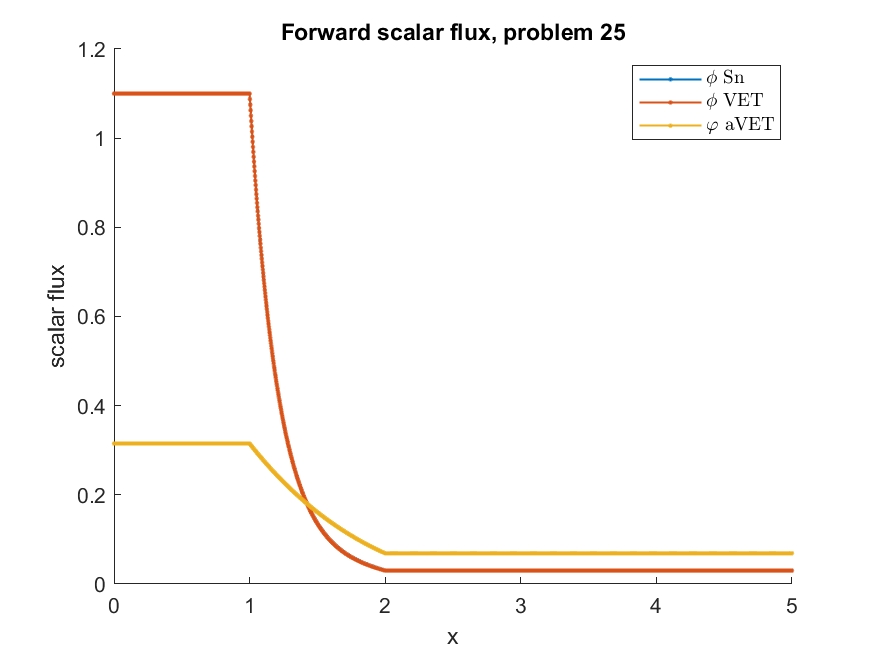
\includegraphics[width=.98\linewidth]{figures2/25phi.png}
  \label{T1:sfig1}
\end{subfigure}
%
\begin{subfigure}{0.45\textwidth}
  \centering
  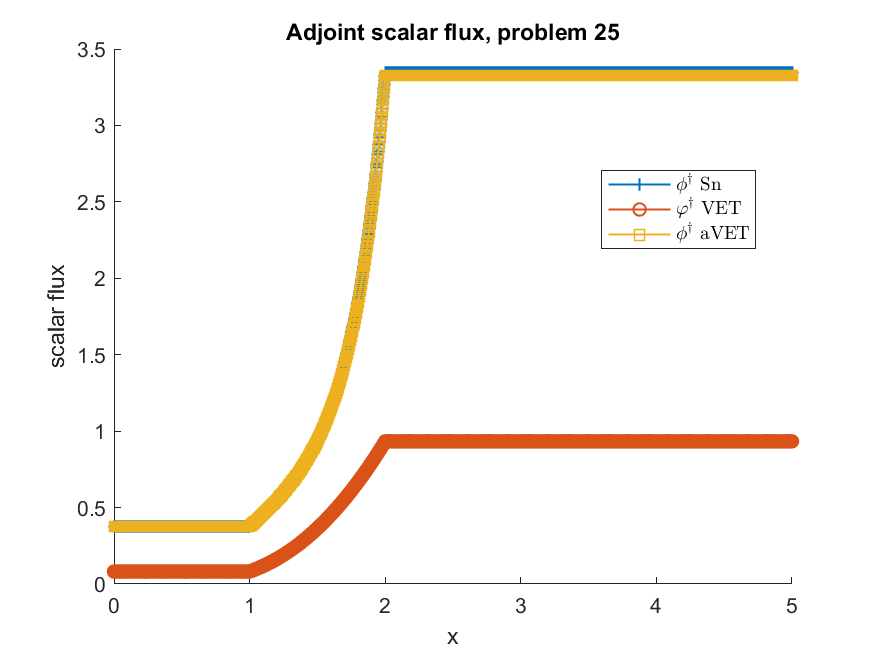
\includegraphics[width=.98\linewidth]{figures2/25phia.png}
  \label{T1:sfig2}
\end{subfigure}
\end{figure}
\end{frame}

 %%%%%%%%%%%%%%%%%%%%%%%%%%%%%%%%%%%%%%%%%%%%%%%%%%%%%%%%%%%%%%%%%%%%%%%%%%%%%%%%%%%%%%%%%%%%%%%%%%%%%%%%%%%
\begin{frame}\frametitle{Shielded Incident Beam}
 \begin{flushleft}

\begin{figure}[H]
\label{Trial4}
\begin{minipage}{.35\textwidth}
\centering
\begin{subfigure}{.45\textheight}
  \centering
  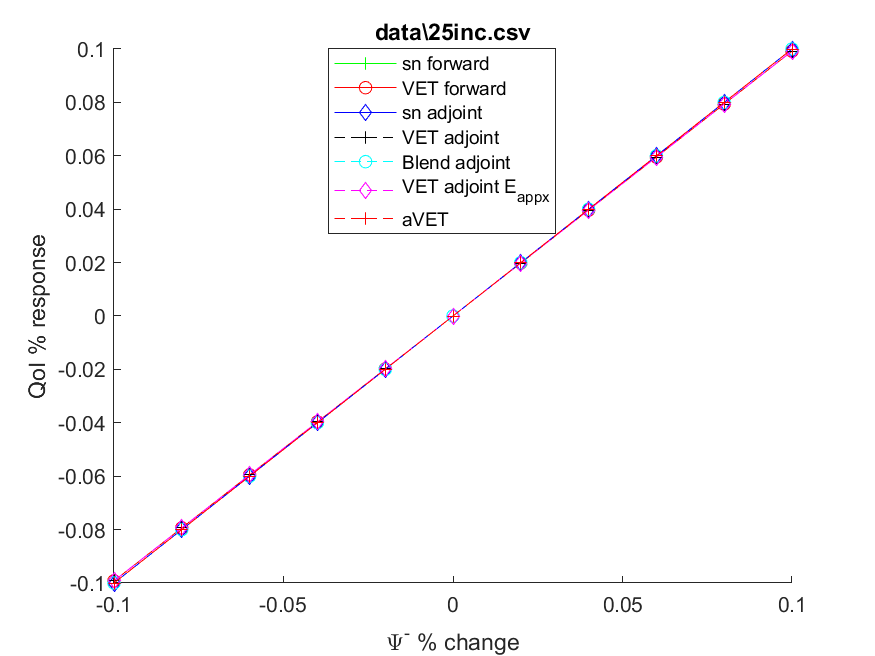
\includegraphics[width=.98\linewidth]{figures2/25incSens.png}
  \label{T1:sfig1}
\end{subfigure}%

\begin{subfigure}{.45\textheight}
  \centering
  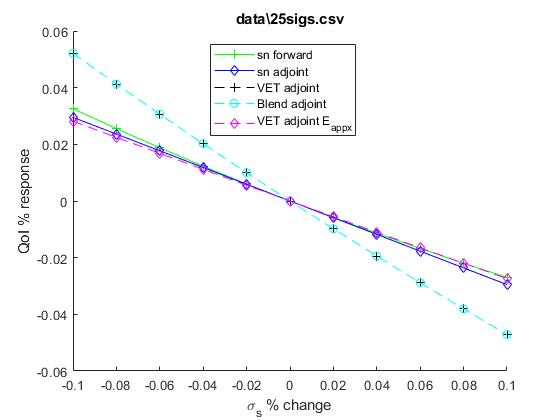
\includegraphics[width=.98\linewidth]{figures2/25sigsSensNoavet.png}
\end{subfigure}
\end{minipage}
\begin{minipage}{.60\textwidth}
\begin{subfigure}{1\textwidth}
  \centering
  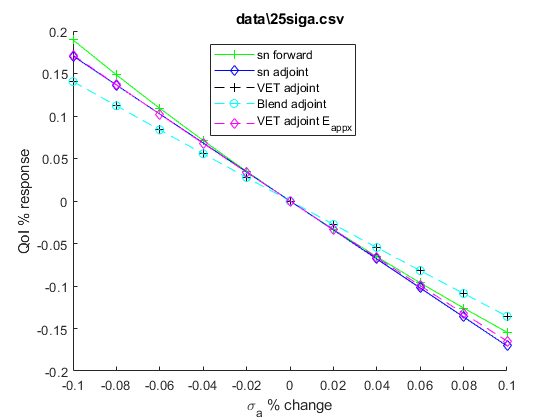
\includegraphics[width=.98\linewidth]{figures2/25sigaSensNoavet.png}
\end{subfigure}%
%\begin{subfigure}{.5\textheight}
%  \centering
%  \includegraphics[width=.98\linewidth]{figures2/25incsigaSens.png}
%\end{subfigure}
\end{minipage}
\end{figure}
\end{flushleft}
\end{frame}

%%%%%%%%%%%%%%%%%%%%%%%%%%%%%%%%%%%%%%%%%%%%%%%%%%%%%%%%%%%%%%%%%%%%%%%%%%%%%%%%%%%%%%%%%%%%%%%%%%%%%%%%%%%

\begin{frame}\frametitle{Shielded Incident Beam}
 \begin{flushleft}
\begin{itemize}
\item VET/blended method was worse for cross section perturbations, particularly scattering, when compared to the isotropic incident.
\item $\delta \Edd$ approximation fared well and nearly reconciled transport adjoint and VET adjoint.
\end{itemize}
\end{flushleft}
\end{frame}

 %%%%%%%%%%%%%%%%%%%%%%%%%%%%%%%%%%%%%%%%%%%%%%%%%%%%%%%%%%%%%%%%%%%%%%%%%%%%%%%%%%%%%%%%%%%%%%%%%%%%%%%%%%%

\begin{frame}\frametitle{Homogeneous System, Homogeneous Perturbation}
 \begin{flushleft}
\begin{table}[H]
\label{TableT1}
\centering
  \begin{tabular}{| l | r | r | r | r |}
    \hline
    Method  &  $+10\% q $  & $-10\% \siga $ & $+10\% \sigs $ & $+10\% q,-10\% \siga$ \\ \hline
     SN Fwd 			&0.39998 &0.44419 &5.7577e-05 & 0.88858\\ \hline
     VET Fwd			&0.39998 &0.44428 &2.7131e-05 &0.88868\\ \hline
     SN Adj			&0.39998 &0.39983 &6.6307e-05 &0.79980\\ \hline
     VET Adj 			&0.39998 &0.39988 &2.8534e-05 &0.79986\\ \hline
     Blended 			&0.39998 &0.39988 &2.8534e-05 &0.79986\\ \hline
     VET $\delta \Edd$ 	&0.39998 &0.39983 &5.9537e-05 &0.79981\\ \hline
     VET Alt			&0.39998 &0.39980  &4.986e-05	 &0.79978\\ \hline
    \end{tabular}
  \caption{Table of selected results for the homogeneous system under homogeneous perturbations. Values given are absolute $\delta \Edd$. }
\end{table}
\end{flushleft}
\end{frame}

\begin{frame}\frametitle{Homogeneous System, Non-Homogeneous Perturbation}
 \begin{flushleft}
\begin{table}[H]
\centering
  \begin{tabular}{| l | r | r | r | r |}
    \hline
    Method  &  $+10\% q $  & $-10\% \siga $ & $+10\% \sigs $ & $+10\% q,-10\% \siga$ \\ \hline
     SN Fwd 			&0.36309 &0.39952 &2.9680e-05 & 0.79915\\ \hline
     VET Fwd			&0.35947 &0.39517 &1.5072e-05 &0.79040\\ \hline
     SN Adj  			&0.36309 &0.36301 &3.4051e-05 &0.72610\\ \hline
     VET Adj 			&0.35947 &0.35941 &1.5733e-05 &0.71888\\ \hline
     Blended 			&0.36309 &0.35941 &1.5733e-05 &0.72250\\ \hline
     VET $\delta \Edd$ 	&0.36287 &0.36290 &3.0640e-05 &0.72586\\ \hline
     VET Alt			&0.36309 &0.36299 &2.6234e-05 &0.72609\\ \hline
    \end{tabular}
  \caption{Table of selected results for the homogeneous system under inhomogeneous perturbations. Values given are absolute $\delta \Edd$. }
\end{table}
\end{flushleft}
\end{frame}

\begin{frame}\frametitle{Shielded Isotropic Flux}
 \begin{flushleft}
\begin{table}[H]
\centering
  \begin{tabular}{| l | r | r | r | r |}
    \hline
    Method  &  $+10\% \psi^- $  & $-10\% \siga $ & $+10\% \sigs $ & $+10\% \psi^-,-10\% \siga$ \\ \hline
     SN Fwd 			&0.023401 &0.021079 &-0.0067476 & 0.046588\\ \hline
     VET Fwd			&0.023181 &0.019670 &-0.0066481 &0.044818\\ \hline
     SN Adj  			&0.023401 &0.019975 &-0.0068956 &0.043376\\ \hline
     VET Adj 			&0.023181 &0.018981 &-0.0067751 &0.042162\\ \hline
     Blended 			&0.023401 &0.018981 &-0.0067751 &0.042381\\ \hline
     VET $\delta \Edd$ 	&0.023181 &0.020070 &-0.0065156 &0.043251\\ \hline
     VET Alt			&0.023401 &0.035869 &-0.012563	&0.059270\\ \hline
    \end{tabular}
  \caption{Table of selected results for the shielding system under perturbations. Values given are absolute $\delta \Edd$. }
\end{table}
\end{flushleft}
\end{frame}

%%%%%%%%%%%%%%%%%%%%%%%%%%%%%%%%%%%%%%%%%%%%%%%%%%%%%%%%%%%%%%%%%%%%%%%%%%%%%%%%%%%%%%%%%%%%%%%%%%%%%%%%%%%%%%%%%%%%%%%%%%%%%%%%%%%%%%%%
\setcounter{framenumber}{\value{finalframe}}

\end{document}